% Chapter Template

\chapter{The Algebra of Integrating Partial Belief Systems} % Main chapter title

\label{chapter5} % Change X to a consecutive number; for referencing this chapter elsewhere, use \ref{ChapterX}

\lhead{Chapter 5. \emph{The Algebra of Integrated Partial Belief Systems}} % Change X to a consecutive number; this is for the header on each page - perhaps a shortened title

%----------------------------------------------------------------------------------------
%	SECTION 1
%----------------------------------------------------------------------------------------

The examples of Section \ref{sec:exalgo} showed that the IDSS's expected utilities are often polynomial functions whose indeterminates are individually delivered by different panels. By requesting only this information, the implementation of an IDSS can become orders of magnitude more manageable. This is because panels just need to communicate a few summaries from their sample: a trivial and fast task to perform. 

Therefore, for the sole purpose of decision support, the full inferential conditions guaranteeing a sound and distributed analysis of Chapter \ref{chapter3} are actually too strict. These can be relaxed whilst retaining the coherence of the IDSS. Taking an algebraic approach, in this chapter we develop  a methodology that ensures coherence in these types of partially defined systems, meaning systems where panels only deliver certain selected summaries. Following \citet{Leonelli2015b}, we first define the new notion of algebraic expected utility of an IDSS. This definition enables us to impose new conditions tailored to the needs of an IDSS concerning the uncorrelatedness of certain polynomials. These conditions, often weaker than panel independence, can guarantee an IDSS is adequate. We discuss how and when it is possible to achieve adequacy in a number of typical frameworks. Importantly, this algebraic approach enables us to extend results about the computation of moments of decomposable functions in DAGs \citep{Cowell1999a, Nilsson2001} for a particular subclass of BN models.  

Although this is not often recognised in the literature, algebraic approaches are intimately linked to symbolic ones, where probabilities are treated as indeterminates in a computer algebra system, thus not requiring an exact numerical specification. Symbolic inference is often used in sensitivity analysis to identify the probabilities a DM needs to be particularly precise about in her specification, as these might drastically change the ranking of the available policies \citep{French2003}. We symbolically define two important instances of models that can be part of an IDSS structural consensus, namely IDs and staged trees. We develop new symbolic inferential techniques for these two models, extending  current literature to both decision and asymmetric problems. An extensive discussion of these results can be found in \citet{Leonelli2015a} and \citet{Gorgen2015}. 

 The structure of the chapter is as follows. In Section \ref{sec:history} we  review the main developments in symbolic and algebraic inferential methods. In Section \ref{sec:description} we  define algebraically the  expected utility of an  IDSS. Section \ref{sec:momind} introduces polynomial conditions the panels' summaries need to entertain and we then show in Section \ref{sec:adequacy1} how these are able to guarantee adequacy and distributivity. Section \ref{sec:parexamples} presents a variety of examples of these methods. In Section \ref{sec:short} we review recent symbolic methods for two particular integrating structures: IDs and staged trees. We conclude with a discussion.
 
\section{A Brief Overview of Symbolic and Algebraic Methods in Statistics}
\label{sec:history}
As mentioned in the introduction, symbolic and algebraic methods for statistical inference have been developed independently by two different community of researchers. Symbolic ones have been the focus of mostly computer scientists, whilst algebraic ones of mathematicians and statisticians. However, in both cases, the probabilities associated to a statistical model are described as polynomials, whose structure is then exploited to study the inferential properties of such models in a variety of applications. 

Symbolic methods focused mostly on graphical models and specifically on BNs, both discrete \citep{Castillo1995,Castillo1997a} and Gaussian \citep{Castillo1997}. Probabilities and moments associated to vertices are thought of as indeterminates of a computer algebra system (such as Maple or Matlab), where the model's probabilities can then be seen as polynomials with such indeterminates.  \citet{Castillo1996a} and \citet{Castillo2003} developed and implemented algorithms for the computation of polynomials associated to the joint probabilities of a BN model. In these works the bounds the probabilities of the vertices of the network have to respect were also identified, and these can then be used in sensitivity analyses. The fundamental idea behind this approach lies in the fact that once the qualitative structure of the model is constructed, numerical specifications of the involved probabilities do not need to be delivered a priori for the algorithms to run. Furthermore the above mentioned bounds inform a DM about probability values that cannot be delivered, thus simplifying the elicitation process. 

However, the symbolic inferential algorithms of \citet{Castillo1997b} had several drawbacks. Most importantly these computed \textit{every} possible monomial deriving from the symbolic definition of the model, only later dropping those associated to non compatible instantiations. This required the computation of the Cartesian product  of the sets of probabilities associated to the vertices of the BN, which can become infeasible as the size of the network grows. In \citet{Darwiche2003} a new symbolic inferential algorithm speeded up the computation of the probability polynomials, by converting the underlying BN into an \textit{Arithmetic Circuit (AC)}. This circuit can then be evaluated through fast routines to output the required polynomials. Importantly, \citet{Darwiche2003} also showed that a large number of probabilistic queries can be answered by computing certain \textit{derivatives} of the probability polynomials, which are then easier to handle because the associated AC has a smaller dimension. Such methods were subsequently extended to DBNs \citep{Brandherm2004}.

Beside the possibility of not having to elicit probabilities before any inference takes place, another great advantage of symbolic approaches is that these methods straightforwardly support various \textit{sensitivity analyses}. In particular users can simply plug-in different numbers into the probability indeterminates and observe how these change the inferential results on a set of goal variables. Alternatively, much more sophisticated sensitivity techniques have now been implemented \citep{Chan2001,Chan2004}. 

Although the computing capability of modern computers is constantly growing, it has been possible to apply symbolic approaches only in small/medium sized applications. This is because each probability specification is treated as an unknown variable in a computer system. This requires much more memory space than a single number. Furthermore, as shown by \citet{Cooper1990}, the number of monomials in BN models grows exponentially with the number of vertices, often making the computation of such polynomials prohibitive. However, we note here that the technology of IDSSs allows us to apply symbolic methods to much larger models. This is because we can define symbolically only the \textit{outputs} of each component DSS, which is the only relevant information an IDSS needs to process. At the same time, this symbolic definition leads straightforwardly to the use of sensitivity analyses for the outputs of IDSSs, which can be extremely useful for building consensus among the panel members. 

The alternative stream of research using polynomial techniques in statistics is usually referred to as \textit{algebraic statistics}. Among others, this uses techniques from algebraic geometry and computational commutative algebra to gain insights into the structure of certain statistical models \citep{Riccomagno2009a}. The first developments of algebraic statistics were on  the use of both Gr\"{o}bner bases in Markov chain sampling algorithms \citep{Diaconis1998} and commutative algebraic techniques in the design and analysis of experiments \citep{Pistone1996}. 

Subsequently, algebraic statistics also started to be applied to more general statistical models. Certain statistical models have been identified with certain algebraic varieties \citep{Pistone2002}. Big part of the research in this area then focused on graphical models, as for example BNs \citep{Garcia2005, Sullivant2008}, MNs \citep{Geiger2006} and trees \citep{Settimi2000}. The number of applications of algebraic methods in statistics is now enormous \citep[see e.g. the monographs,][]{Gibilisco2010, Pistone2002, Drton2009b, Pachter2005}.

To our knowledge, the methods we develop in the following sections are the first application of symbolic and algebraic techniques to Bayesian decision analysis.  

\section{An Algebraic Description of Integrating Systems}
\label{sec:description}
The computation of the expected utilities in the examples of Section \ref{sec:exalgo} showed the difficulty of identifying the beliefs that need to be delivered  to the IDSS by panels. The situation becomes even more complicated when the utility consensus includes multilinear or multiplicative utility factorisations introduced in Definitions \ref{def:multilinear} and \ref{def:multiplicative} respectively (unless all panels can simply define independent marginal models for the variables under their jurisdiction). 

Approaching the problem from an algebraic viewpoint allows us to identify the necessary panels' summaries and the required assumptions for adequacy. In order to do this we first need to define the expected utility polynomials. Recall that there are $m $ panels of experts $\{G_i:i\in[m]\}$, $[m]=\{1,\dots,m\}$, each delivering beliefs about $\bm{\theta}_i$, $i\in[m]$, parametrising the density of $\bm{Y}_i\;|\;\bm{d}$, for a decision $\bm{d}\in\bm{\mathcal{D}}$. The conditional expected utility is $\bar{u}(\bm{d}\;|\;\bm{\theta})$, whilst $\bar{u}(\bm{d})$ is the expected utility.

\begin{definition}
The conditional expected utility $\bar{u}(\bm{d}\;|\;\bm{\theta})$ of an IDSS is called \textbf{algebraic} if, for each $\bm{d}\in \bm{\mathcal{D}}$ and $\bm{\theta} \in \bm{\Theta} $, $\bar{u}(\bm{d}\;|\;\bm{\theta})$ is a square-free polynomial 
\[
\bar{u}(\bm{d}\;|\;\bm{\theta})=f_{\bm{d}}\left( \bm{\lambda}_{1}(\bm{\theta}_{1},\bm{d}),\cdots,\bm{\lambda}_m(\bm{\theta }_{m},\bm{d})\right) 
\]
 in functions $\bm{\lambda }_{_{i}}(\bm{\theta }_{i},\bm{d})$ of the parameters $\bm{\theta }_{_{i}}$ of panel $G_{i}$, $i\in[m]$.
\end{definition}

We now explicitly define the algebraic conditional expected utilities $f_{\bm{d}} $. Let $\bm{\lambda}_i(\bm{\theta}_i,\bm{d})=(\lambda _{ji}(\bm{\theta }_{i},\bm{d}))^\T_{j\in[s_i]}$, for an $s_i\in\mathbb{Z}_{\geq 1}$, and $\bm{b}\in B=\bigtimes_{i\in[m]}B_{i}$ , where $B_{i}=[s_i]^0=[s_i]\cup \{0\}$, $i\in[m]$. For a given $\bm{b}$, let $i\in B_j$ be its j-th entry and let $b(j,i)=0$ if $j\neq i$, $b(j,i)=1$ if $j=i$ and $b(0,i)=1$, for $i\in[m]$ and $j\in[s_i]$. Then, if we define $\lambda_{0i}(\bm{\theta}_i,\bm{d})=1$, for every $\bm{\theta}_i\in \bm{\Theta}_i$, $\bm{d}\in\bm{\mathcal{D}}$ and $i\in[m]$, we can write 
\begin{equation}
f_{\bm{d}}\left( \bm{\lambda }_{_{1}}(\bm{\theta }_{1},\bm{d}),\dots,\bm{\lambda }_{m}(\bm{\theta }_{m},\bm{d})\right)  = \sum_{\bm{b}\in B}k_{\bm{b},\bm{d}}\lambda _{\bm{b}}(\bm{ \theta },\bm{d}),  \label{algebraic utility} \end{equation}
where
\begin{equation*}
 \lambda _{\bm{b}}(\bm{\theta },\bm{d}) = \prod_{i\in[m]}\prod_{j\in[s_i]^0}\lambda_{ji}(\bm{\theta }_{i},\bm{d})^{b(j,i)},  \label{eq:aceu2}
\end{equation*}
is a monomial, having at most one term not unity delivered by each panel. So in particular, $f_{\bm{d}} $ is a square-free polynomial. For a given $\bm{b}\in B$, let
\begin{equation*}
\mu _{ji}(\bm{d})= \mathbb{E}\left( \lambda_{ji}(\bm{\theta }_{i},\bm{d})^{b(j,i)}\right). 
\end{equation*}

For the distributivity of the IDSS we need the following property.
\begin{definition}
Call an IDSS \textbf{score separable} if, in the notation above, the collective agrees that, for all decisions $\bm{d}\in \bm{\mathcal{D}}$ and all indices $\bm{b}\in B$ such that $k_{\bm{b},\bm{d}}\neq 0$,
\begin{equation}
\mathbb{E}\left( \lambda _{\bm{b}}(\bm{\theta },\bm{d})\right)=\prod_{i\in[m]}\prod_{j\in[s_i]^0}\mu_{ji}(\bm{d}). \label{uncor}
\end{equation}
\label{def:scoresep}
\end{definition}
 Let, for every $\bm{d}\in\bm{\mathcal{D}}$, $\bm{\mu }_{i}(\bm{d})=\left( \mu _{ji}(\bm{d})\right)^\T_{j\in[s_i]}$. A consequence of the definitions above is the following. 

\begin{lemma}
\label{lemma:ciao}
Suppose panel $G_{i}$ delivers its vectors of expectations $\bm{\mu }_{i}(\bm{d})$, $i\in[m]$, $\bm{d}\in\bm{\mathcal{D}}$, to the SB. Then, under the collective assumptions of an algebraic conditional expected utility, if the IDSS is score separable then it is  adequate.
\end{lemma}
\begin{proof}
The definition of adequacy in Definition \ref{def:adequacy} means in this framework that the expected utility $\bar{u}(\bm{d})$ is a function of $\mu_{ji}(\bm{d})$ and $k_{\bm{b},\bm{d}}$ only, for $i\in[m]$, $j\in[s_i]^0$, $\bm{b}\in B$ and $\bm{d}\in\bm{\mathcal{D}}$.  Now note that 
\begin{equation*}
\bar{u}(\bm{d})=\E\left(f_{\bm{d}}\left( \bm{\lambda }_{_{1}}(\bm{\theta }_{1},\bm{d}),\dots,\bm{\lambda }_{m}(\bm{\theta }_{m},\bm{d})\right)\right)= \sum_{\bm{b}\in B}k_{\bm{b},\bm{d}}\E\left(\lambda _{\bm{b}}(\bm{ \theta },\bm{d})\right).\label{eq:nonso}
\end{equation*}
The definition of score separability in equation (\ref{uncor}) then implies that 
\begin{equation*}
\bar{u}(\bm{d})=\sum_{\bm{b}\in B}k_{\bm{b},\bm{d}} \prod_{i\in[m]}\prod_{j\in[s_i]^0}\mu_{ji}(\bm{d}),
\end{equation*}
from which the lemma follows.
\end{proof}

 We can therefore deduce from Lemma \ref{lemma:ciao} that adequacy is guaranteed whenever score separability holds, under the assumption of an algebraic conditional expected utility. In the following section we introduce conditions that ensure this type of separability. We then identify classes of models that give rise to algebraic conditional expected utilities.

\section{Moment and Partial Independence}
\label{sec:momind}
Equation (\ref{uncor}) together with Lemma \ref{lemma:ciao} shows that adequacy is guaranteed whenever the expectation of certain functions of the panels' parameters separate appropriately. We introduce now a new type of independence called \textit{partial independence}.
\begin{definition}
\label{def:partial}
Let $f_{\bm{d}}(\bm{\lambda }_{_{1}}(\bm{\theta }_{1},\bm{d}),\dots,\bm{\lambda }_{m}(\bm{\theta }_{m},\bm{d}))$ be the algebraic conditional expected utility of an IDSS. We say that an IDSS is \textbf{partially independent} if 
\begin{equation*}
\E(f_{\bm{d}}(\bm{\lambda }_{_{1}}(\bm{\theta }_{1},\bm{d}),\dots,\bm{\lambda }_{m}(\bm{\theta }_{m},\bm{d})))=f_{\bm{d}}(\E(\bm{\lambda }_{_{1}}(\bm{\theta }_{1},\bm{d})),\dots,\E(\bm{\lambda }_{m}(\bm{\theta }_{m},\bm{d}))).
\end{equation*}
\end{definition}
This condition requires the expectation of the product of certain functions of the parameters overseen by different panels to be equal to the product of the individual expectations.

Often the $\lambda_{ji}$, $i\in[m]$, $j\in[s_i]$, are monomial functions of the panels' parameters. It is therefore helpful to introduce the following independence condition specific for monomial functions. Let $<_{lex}$ denote a lexicographic order (see Appendix \ref{appendixC}).

\begin{definition}
\label{def:moment}
Let $\bm{\theta}=(\theta_i)^\T_{i\in[n]}\in\mathbb{R}^{n}$ be a parameter vector and $\bm{b}=(b_i)^\T_{i\in[n]}\in\mathbb{Z}^n_{\geq 0}$. We say that $\bm{\theta}$ entertains \textbf{moment independence} of order $\bm{b}$ if,  $\forall~\bm{b}'=\left(b_i'\right)_{i\in[n]}^\T\leq_{lex} \bm{b}$, 
\begin{equation*}
\E\left(\bm{\theta}^{\bm{b}'}\right)=\prod_{i\in[n]}\E\left(\theta_i^{b_i'}\right).
\end{equation*}
\end{definition}

It is generally well known that standard probabilistic independence only guarantees that the \textit{first} moment of a product can be written as the product of the moments. Separations for higher orders are implied by standard independence only through a cumulant parametrisation, where the cumulant generating function for a product of independent random variables (defined as a random sum of independent realisations) is the composition of the respective cumulant generating functions.

For the purpose of decision support in partial belief systems it is helpful to study moments, since expected utilities often formally depend on these. Consider for instance two parameters $\theta_1$ and $\theta_2$. Suppose a conditional expected utility is equal to $\theta_1^2\theta_2^2$ and that a moment independence of order $(2,2)$ holds. Then,
\begin{equation}
\mathbb{E}\left(\theta_1^2\theta_2^2\right)=\mathbb{E}\left(\theta_1^2\right)\mathbb{E}\left(\theta_2^2\right)=\mathbb{E}(\theta_1)^2\mathbb{E}(\theta_2)^2+\mathbb{E}(\theta_1)^2\mathbb{V}(\theta_2)+\mathbb{E}(\theta_2)^2\mathbb{V}(\theta_1)+\mathbb{V}(\theta_1)\mathbb{V}(\theta_2).
\label{eq:towerex}
\end{equation}
The same expression is obtained when using sequentially the tower rule of expectations and the law of total variance of Proposition \ref{prop:towerrules} under the assumption of independence of the two parameters above. Therefore, the expression obtained under moment independence is reasonable and coincides with the one implied by the independence of $\theta_1$ and $\theta_2$. However the condition we need for equation (\ref{eq:towerex}) to hold \textit{does not require} $\theta_1$ and $\theta_2$ to be independent. 

\section{Adequacy in Partially Defined Systems}
\label{sec:adequacy1}

 Given the definitions of new independence concepts tailored for IDSSs, we can now study in which cases adequacy holds. The following result easily follows from the definition of partial independence.
 
\begin{lemma}
\label{lemma:ciaociao}
Suppose $f_{\bm{d}}(\bm{\lambda }_{_{1}}(\bm{\theta }_{1},\bm{d}),\dots,\bm{\lambda }_{m}(\bm{\theta }_{m},\bm{d}))$ is the algebraic conditional expected utility of an IDSS and that partial independence is in the structural consensus. The IDSS is then adequate if panel $G_i$ delivers the expectations $\bm{u}_i(\bm{d})$, $i\in[m]$, $\bm{d}\in\bm{\mathcal{D}}$.
\end{lemma}
\begin{proof}
This result easily follows by noting that partial independence implies score separability. Specifically,
\begin{eqnarray*}
\bar{u}(\bm{d})&=&\E\left(f_{\bm{d}}(\bm{\lambda }_{_{1}}(\bm{\theta }_{1},\bm{d}),\dots,\bm{\lambda }_{m}(\bm{\theta }_{m},\bm{d}))\right)=f_{\bm{d}}(\E(\bm{\lambda }_{_{1}}(\bm{\theta }_{1},\bm{d})),\dots,\E(\bm{\lambda }_{m}(\bm{\theta }_{m},\bm{d})))\\
&=&\sum_{\bm{b}\in B}k_{\bm{b},\bm{d}} \prod_{i\in[m]}\prod_{j\in[s_i]^0}\mu_{ji}(\bm{d}).
\end{eqnarray*}
The result then follows from Lemma \ref{lemma:ciao}.
\end{proof}

Assuming the conditional expected utility is a polynomial in the panels' parameters, then under a specific moment independence assumption we have the following. 

\begin{lemma}
\label{lemma:ciao3}
Assume $f_{\bm{d}}(\bm{\lambda }_{_{1}}(\bm{\theta }_{1},\bm{d}),\dots,\bm{\lambda }_{m}(\bm{\theta }_{m},\bm{d}))$ is the algebraic conditional expected utility of an IDSS, $\bm{\theta}_i=(\theta_{ji})^\T_{j\in[s_i]}$ and $\lambda_{ji}(\bm{\theta}_i,\bm{d})=\bm{\theta}_{i}^{\bm{a}_{ji}}$, with $\bm{a}_{ji}\in\mathbb{Z}_{\geq 0}^{s_i}$, $i\in[m]$, $j\in[s_i]$. Let $\bm{a}^*_i=({a_{ji}^*})_{j\in[s_i]}^\T$, where $a_{ji}^*$ is the greatest element in $\{a_{ji}:j\in[s_i]\}$, $i\in[m]$, and let ${\bm{a}^*}^\T=({\bm{a}_i^*}^\T)_{i\in[m]}$. Let $\bm{\theta}=(\bm{\theta}_i^\T)_{i\in[m]}^\T$ and assume the structural consensus includes the assumption that $\bm{\theta}$ entertains moment independence of order $\bm{a}^*$. Then the IDSS is adequate if panel $G_i$ delivers  the vectors of expectations $\bm{u}_i(\bm{d})$, $i\in[m]$, $\bm{d}\in\bm{\mathcal{D}}$.
\end{lemma} 
\begin{proof}
Adequacy is again guaranteed if the expected utility function can be written in terms of $\mu_{ji}(\bm{d})$, $i\in[m]$, $j\in[s_i]$ and $\bm{d}\in\bm{\mathcal{D}}$. Note that
\begin{eqnarray*}
\bar{u}(\bm{d})&=&\E\left(f_{\bm{d}}(\bm{\lambda }_{_{1}}(\bm{\theta }_{1},\bm{d}),\dots,\bm{\lambda }_{m}(\bm{\theta }_{m},\bm{d}))\right)=\sum_{\bm{b}\in B}k_{\bm{b},\bm{d}}\E\left( \prod_{i\in[m]}\prod_{j\in[s_i]^0}\lambda_{ji}(\bm{\theta }_{i},\bm{d})^{b(j,i)}\right)\\
&=&\sum_{\bm{b}\in B}k_{\bm{b},\bm{d}}\E\left(\prod_{i\in[m]}\prod_{j\in[s_i]^0}\bm{\theta}_i^{\bm{a}_{ji}}\right).
\end{eqnarray*}
The argument of this expectation is then a monomial of multi-degree lower or equal to $\bm{a}^*$ with respect to a lexicographic order. Moment independence then implies that 
\begin{equation*}
\bar{u}(\bm{d})=\sum_{\bm{b}\in B}k_{\bm{b},\bm{d}}\prod_{i\in[m]}\prod_{j\in[s_i]^0}\mu_{ji}(\bm{d}),
\end{equation*}
and the result follows.
\end{proof}

Both Lemma \ref{lemma:ciaociao} and \ref{lemma:ciao3} start with the assumption of an algebraic conditional expected utility. This is the case for many of the examples we consider in Section \ref{sec:parexamples}. However, we are able to identify families of utility factorisations and statistical models that ensure the associated conditional expected utility is algebraic.  We first introduce two families of utilities that factorise according to the construction of the panels.
\begin{definition}
\label{def:panelsep}
Let $\bm{Y}_i$ be the vector overseen by panel $G_i$, $i\in[m]$, and $\bm{R}_i$ be a function of $\bm{Y}_i$ and $\bm{d}\in\bm{\mathcal{D}}$ only. A multilinear factorisation over $\bm{R}_1,\dots,\bm{R}_m$ is called \textbf{panel separable}.   
\end{definition}

\begin{definition}
Under the conditions of Definition \ref{def:panelsep}, an additive factorisation over $\bm{R}_1,\dots, \bm{R}_m$ is called \emph{additive panel separable}.
\end{definition}

Both families of panel separable and additive panel separable utilities can be seen as a particular instance of a compatible utility factorisation in Definition \ref{compatible}. 

The probabilistic model class we consider here is a generalisation of the DAG linear regressions in equation (\ref{eq:GausBN}) to generic polynomial functions. Henceforth we call these a \textit{polynomial Structural Equation Model (SEM)} \citep[see e.g.][]{Bollen1998,Ullman2003,Wall2000}. SEMs are widely used, especially recently, in the causal literature \citep{Pearl2000}. 

\begin{definition}
\label{def:polystrut}
Let $\bm{Y}=(Y_i)^\T_{i\in[n]}$ be a random vector. A \textbf{polynomial SEM} is defined by, for $i\in[n]$,
\begin{equation*}
Y_i=\sum_{\bm{b}_i\in B_i}\theta_{i\bm{b}_i}\bm{Y}_{[i-1]}^{\bm{b}_i}+\varepsilon_i,
\end{equation*}
where $B_i\subset \mathbb{Z}^{i-1}_{\geq 0}$, $\varepsilon_i$ is an error with mean zero and variance $\psi$, and $\theta_{i\bm{b}_i}$ is a parameter, $i\in[n]$, $\bm{b}_i\in B_i$.
\end{definition}

An alternative formulation of the model in Definition \ref{def:polystrut} in terms of distributions is,  
\begin{equation*}
Y_i\;|\;\bm{\theta}_i,\bm{Y}_{[i-1]}\sim \Big(\sum_{\bm{b}_i\in B_i}\theta_{i\bm{b}_i}\bm{Y}_{[i-1]}^{\bm{b}_i},\psi_i\Big),
\end{equation*}
where $\bm{\theta}_i=(\psi_i,\theta_{i\bm{b}_i})^\T_{\bm{b}_i\in B_i}$ and $i\in[n]$.

Note that these models are suitable candidates for a CK-class since their definition is qualitative in nature.
 
For polynomial SEMs and panel separable utilities, the following holds.
\begin{theorem}
\label{theo:ciao}
Suppose $\bm{R}=\bm{Y}$ and assume panel $G_i$ is responsible for $Y_i$, $i\in[n]$. Assume that the utility consensus of an IDSS includes a panel separable utility and that the structural consensus includes a polynomial SEM. Suppose each panel agreed to model its marginal utility as a polynomial utility function. Then if panels are partially independent, the IDSS is score separable.
\end{theorem}

The proof of this result can be found in Appendix \ref{proof:theociao}.

Theorem \ref{theo:ciao} together with Lemma \ref{lemma:ciao} can be thought of as an instance of the important Theorem \ref{theo:gold}, specifically addressing adequacy in partial belief systems. An IDSS whose CK-class embeds the assumptions of Theorem \ref{theo:ciao} is able to uniquely compute expected utility scores from the individual judgements of the panels. 

Note that, by construction, the partial independence condition of Theorem \ref{theo:ciao} actually corresponds  to a moment independence. The order of such an independence depends on the polynomial form of both the SEM and the utility function. In Section \ref{sec:bn1} we  identify the order of the moment independence condition required for adequacy for a subclass of polynomial SEMs.

\section{Examples}
\label{sec:parexamples}
\subsection{Discrete Models}
\subsubsection{Independence Binary Models.}
We begin with a rather obvious setting where a small number of summaries are sufficient to determine an expected utility maximising decision. Let the CK-class specify that $\bm{R}=\bm{Y}=(Y_i)_{i\in[n]}^\T$, where each variable $Y_i$ is binary and overseen by panel $G_i$. Assume the CK-class includes the belief that $\independent_{i\in[n]} Y_i\;|\; \bm{\theta},\bm{d}$, where $\bm{\theta}=(\theta_i)_{i\in[n]}^\T$ and that $\theta_i$ can be read as the probability $\mathbb{P}(Y_i=1\;|\;\theta_i,\bm{d})$, whatever decision $\bm{d}\in\bm{\mathcal{D}}$ is made, $i\in[n]$. We have already discussed in Section \ref{sec:indadd} how independence models can be part of the structural consensus of a CK-class. 

As in the example in Section \ref{sec:adequacy}, suppose each panel $G_i$ delivers the set of beta distributions $\Be(p_i,q_i)$ for $\theta_i\;|\;\bm{d}$, $i\in[n]$.  Assume further the CK-class includes utility factorisations of the form
\begin{equation*}
\label{eq:ind1}
u(y_1,\dots, y_n)=\sum_{i\in[n]}k_iy_i+\sum_{i\in[n]}\sum_{j\in[n]_i}k_{ij}y_iy_j.
\end{equation*}
With no further assumptions, the conditional expected utility can be written as
\begin{equation}
\label{eq:ind2}
\bar{u}(\bm{d}\;|\;\bm{\theta})=\sum_{i\in[n]}k_i\lambda_i(\theta_i,\bm{d})+\sum_{i\in[n]}\sum_{j\in[n]_i}k_{ij}\lambda_i(\theta_i,\bm{d})\lambda_j(\theta_j,\bm{d}),
\end{equation}
where $\lambda_i(\theta_i,\bm{d})=\theta_i$, $[n]_i=\{i+1,\dots,n\}$. Thus,  equation (\ref{eq:ind2}) is an algebraic conditional expected utility. In this example  partial independence then corresponds to moment independence of order $\bm{1}$, where $\bm{1}$ is a vector of dimension $n$ with $1$ in all its entries. In this case, partial independence is implied by panel independence. Furthermore all the monomials $\lambda_{\bm{b}}(\bm{\theta},d)$ formally defined in equation (\ref{algebraic utility}) here are monomials of degree  either  one or two corresponding respectively to $\lambda_i(\theta_i,\bm{d})$ or $\lambda_i(\theta_i,\bm{d})\lambda_j(\theta_j,\bm{d})$, for $i\in[n]$ and $j\in[n]_i$.

Now let $\mu_i=p_i(p_i+q_i)^{-1}=\mathbb{E}(\theta_i\;|\;\bm{d})$ and assume partial independence is in the CK-class. We can see that taking the expectation of equation (\ref{eq:ind2}) we have that
\begin{equation*}
\label{eq:ind3}
\bar{u}(\bm{d})=\sum_{i\in[n]}k_i\mu_i+\sum_{i\in[n]}\sum_{j\in[n]_i}k_{ij}\mu_i\mu_j,
\end{equation*}
where $\bar{u}(d)$ is the expected utility. Thus this IDSS is adequate. Note that this IDSS does not need panel independence to uniquely compute expected utility scores, but only a simple moment independence. 


\subsubsection{Staged Trees.}
Consider now the staged tree in Figure \ref{fig:ET} of Section \ref{sec:tree}, that we report again on page \pageref{riporto} for convenience. As discussed in Section \ref{sec:IDSSET}, staged trees can be part of a coherent IDSS whenever panels oversee disjoint subsets of either the position set or the stage set. Recall that this tree has four stages (coinciding with its positions) $w_0=\{v_0\},$ $w_1=\{v_1\}$, $w_2=\{v_2\}$ and $w_3=\{v_3,v_4\}$. Suppose there are three panels $G_1$, $G_2$ and $G_3$ having responsibility over $w_0$, $\{w_1,w_2\}$ and $w_3$ respectively.

\begin{figure}
\centerline{
\hspace*{-16mm} \xymatrixrowsep{0.5pc}{\xymatrixcolsep{2pc}
\xymatrix{
&&&&\bullet~v_{7}\\
&&&\bullet~v_{3}\ar@[red][r]_{\text{no}}\ar@[blue][ru]^{\text{yes}}&\bullet~v_{8}\\
&&\bullet~v_{1}\ar[r]_{\text{low}}\ar[ru]^{\text{high}}&\bullet~v_{4}\ar@[blue][r]|{\text{yes}}\ar@[red][rd]_{\text{no}}&\bullet~v_{9}\\
v_0\hspace*{-16mm}&\bullet\ar[ru]^{\text{yes}}\ar[rd]_{\text{no}}&&&\bullet~v_{10}\\
&&\bullet~v_{2}\ar[r]^{\text{high}}\ar[rd]_{\text{low}}&\bullet~v_{5}\\
&&&\bullet~v_{6}
}}}
\label{riporto}
\end{figure}

In the notation of Example \ref{ex:staged}, assume the collective has agreed on an additive utility factorisation such that 
\[
u(y_1,y_2,y_3)=k_1u_1(y_1)+k_2u_2(y_2)+k_3u_3(y_3),
\]
where $Y_1,Y_2,Y_3$ are the variables in the associated BN representation of this tree, and that they have been jointly able to further specify the criterion weights.  Label the outcomes of this tree with a $1$ for yes and high, whilst a $0$ denotes no and low outcomes. Let $\psi_{ij}=u_i(j)$, where $j\in\{0,1\}$, and recall that $\theta_{ss'}=\mathbb{P}(Y_s=s'\;|\;\bm{\theta},\bm{d})$, for a situation $s\in S(\mathcal{T})$, $s'\in\mathcal{Y}_s=\{1,0\}$ and $\bm{d}\in\bm{\mathcal{D}}$, where $\bm{\theta}$ is the overall parameter vector. In this parametrisation, the staged tree in Figure \ref{fig:ET} introduces the constraints $\theta_{31}=\theta_{41}$ and $\theta_{30}=\theta_{40}$, where for example $\theta_{31}=\mathbb{P}(Y_3=\text{yes}\;|\; Y_2=\text{high}, Y_1=\text{yes},\bm{\theta},\bm{d})$.

Through a sequential application of the tower rule of expectation, it can be easily deduced that the conditional expected utility of this problem can be written as
\begin{equation}
\label{eq:staged2}
\bar{u}(\bm{\theta}\;|\;\bm{d})=\bar{u}_1+\bar{u}_2+\bar{u}_{3},
\end{equation}
where
\begin{align}
\begin{split}
\label{eq:staged3}
&\bar{u}_1=k_1\psi_{11}\theta_{01}+k_1\psi_{10}\theta_{00},\\
&\bar{u}_2=k_2\psi_{21}\theta_{11}\theta_{01}+k_2\psi_{20}\theta_{10}\theta_{01}+k_2\psi_{21}\theta_{21}\theta_{00}+k_2\psi_{20}\theta_{20}\theta_{00},\\
&\bar{u}_{3}=k_3\psi_{31}\theta_{31}\theta_{11}\theta_{01}+k_3\psi_{30}\theta_{30}\theta_{11}\theta_{01}+k_3\psi_{31}\theta_{41}\theta_{10}\theta_{01}+k_3\psi_{30}\theta_{40}\theta_{10}\theta_{01}.
\end{split}
\end{align}

So the conditional expected utility in equations (\ref{eq:staged2})-(\ref{eq:staged3}) is again algebraic. The coefficients $k_{\bm{b},\bm{d}}$ of the monomials in equation (\ref{algebraic utility}) correspond to the jointly agreed criterion weights, and the unknown functions $\bm{\lambda}_{i}(\bm{\theta}_i,\bm{d})$ are as follows 
\begin{align*}
\bm{\lambda}_1(\bm{\theta}_1,\bm{d})&=(\psi_{11}\theta_{01},\psi_{10}\theta_{00})^\T,\\
\bm{\lambda}_2(\bm{\theta}_2,\bm{d})&=(\theta_{11},\theta_{10},\theta_{21},\theta_{20},\psi_{21}\theta_{11},\psi_{20}\theta_{10},\psi_{21}\theta_{21},\psi_{20}\theta_{20})^\T,\\
\bm{\lambda}_3(\bm{\theta}_3,\bm{d})&=(\psi_{31}\theta_{31},\psi_{30}\theta_{30})^\T.
\end{align*}
Thus once more these polynomials are a simple multilinear function of probabilities delivered by different panels. Under partial independence, as guaranteed by  Lemma \ref{lemma:ciao}, an IDSS so defined is adequate. 
 
\subsection{Bayesian Networks}
\label{sec:bn1}

We now consider the BN model class, where each variable of the network is defined as the DAG linear regression introduced in  Definition \ref{def:linreg}. Note that this is an instance of the polynomial SEM of Definition \ref{def:polystrut}. We refer to this model as a \textit{linear SEM} over a DAG $\Gr$.  Although such a model is often multivariate Gaussian, in general this does not have to be the case.

Just as \citet{Sullivant2008}, we consider regression parameters as indeterminates in a polynomial function. We associate these to edges and vertices of the underlying DAG. Let $\Gr$ be a DAG with vertex set $V(\Gr)=\{Y_i:i\in[n]\}$ and let, for $i\in[n]$, $\theta_{0i}'=\theta_{0i}+\varepsilon_{i}$ be the indeterminate associated to the vertex $Y_i$, whilst $\theta_{ij}$, for $(Y_i,Y_j)\in E(\Gr)$, is the indeterminate associated to the corresponding edge.\footnote{We think of $\theta_{0i}'$ as a parameter although this consists of the sum of a parameter and an error. Note however that from a Bayesian viewpoint these are  both random variables.} Define $\vec{P}_i$ as the set of rooted directed paths (see Appendix \ref{appendixB}) in $\Gr$ ending in $Y_i$. For every element $P\in\vec{P}_i$ we define $\bm{\theta}_P$ as
 \begin{equation*}
 \bm{\theta}_P=\prod_{Y_i\in P}\theta_{0i}'\prod_{(Y_i,Y_j)\in P}\theta_{ij},
 \end{equation*}
and we call $\bm{\theta}_{P}$ the \textit{path monomial}.

\begin{example}
Consider the DAG in Figure \ref{fig:BNexample}. The set $\vec{P}_3$ for instance is equal to
\begin{equation}
\label{eq:paths}
\{(Y_3),(Y_2,(Y_2,Y_3)), (Y_1,(Y_1,Y_3)), (Y_1,(Y_1,Y_2),(Y_2,Y_3))\},
\end{equation}
and $\theta_{03}'$, $\theta_{02}'\theta_{23}$, $\theta_{01}'\theta_{13}$ and $\theta_{01}'\theta_{12}\theta_{23}$ are the corresponding path monomials.
\end{example}

For the purpose of this section we call \textit{algebraic substitution} the process of plugging-in the linear regression definition of a random variable of the DAG into the structural equation definition of the child variable. To illustrate this process, we present now an example of what we mean by an algebraic substitution. 

\begin{example}
Consider again the DAG in Figure \ref{fig:BNexample}. For this network the variables are defined as
\begin{equation*}
\begin{array}{lccl}
Y_4=\theta_{04}+\theta_{14}Y_1+\varepsilon_1, &&& Y_3=\theta_{03}+\theta_{13}Y_1+\theta_{23}Y_2+\varepsilon_3,\\
Y_2=\theta_{02}+\theta_{12}Y_1+\varepsilon_2,&&& Y_1=\theta_{01}+\varepsilon_1.
\end{array}
\end{equation*}
An algebraic substitution of the variables in the definition of $Y_3$ entails
\begin{align}
Y_3&=\theta_{03}+\theta_{13}(\theta_{01}+\varepsilon_1)+\theta_{23}(\theta_{02}+\theta_{12}Y_1+\varepsilon_2)+\varepsilon_3\nonumber\\
&=\theta_{03'}+\theta_{13}\theta_{01}'+\theta_{23}\theta_{02}'+\theta_{23}\theta_{12}Y_1.\label{eq:y3}
\end{align}
Note that an additional algebraic substitution can be performed in equation (\ref{eq:y3}) so that 
\begin{equation}
Y_3=\theta_{03}'+\theta_{13}\theta_{01}'+\theta_{23}\theta_{02}'+\theta_{23}\theta_{12}\theta_{01}'.\label{eq:y3'}
\end{equation}
\end{example}
It is of special interest that after this substitution $Y_3$ is now uniquely defined in equation (\ref{eq:y3'}) in terms of regression parameters. The following proposition formalises that this is in general the case for any variable of a DAG defined as a linear SEM.

\begin{proposition}
\label{prop:algsub}
Let $\Gr$ be a DAG with vertex set $\{Y_i:i\in[n]\}$, whose variables are defined as a linear SEM. Then through algebraic substitutions each variable $Y_i$, $i\in[n]$, can be written as
\begin{equation*}
Y_i=\sum_{P\in\vec{P}_i}\bm{\theta}_{P}.
\end{equation*}
\end{proposition}
\begin{proof}
We prove this result via induction over the indices of the variables. The variable $Y_1$ is by construction a root of the DAG $\Gr$. Thus $Y_1=\theta_{01}'$, where $\theta_{01}'$ is the monomial associated to the only rooted path ending in $Y_1$, namely $(Y_1)$. Assume the result is true for $Y_{n-1}$ and consider $Y_{n}$. By construction and by the inductive hypothesis we have that  
\begin{equation}
Y_{n}=\theta_{0n}'+\sum_{i\in \Pi_n}\theta_{in}Y_i=\theta_{0n}'+\sum_{i\in \Pi_n}\theta_{in}\sum_{P\in \vec{P}_i}\bm{\theta}_P.
\label{eq:pathid}
\end{equation}
Note that every rooted path ending in $Y_n$ is either $(Y_n)$ or consists of a rooted path ending in $Y_i$, $i\in \Pi_n$, together with the edge $(Y_i,Y_n)$. From this observation the result then follows by rearranging the terms in equation (\ref{eq:pathid}).
\end{proof}
\begin{example}
Equation (\ref{eq:y3'}) shows that $Y_3$ can be written as the sum of the monomials associated to each rooted path ending in $Y_3$, where the set of rooted paths is in equation (\ref{eq:paths}).
\end{example}

An algebraic substitution corresponds to computing the conditional expectation of a random variable. This result is formalised by the following proposition.

\begin{proposition}
\label{prop:condex}
Let $\bm{\theta}^\T=(\bm{\theta}_i^\T)$, where $\bm{\theta}_{i}=(\theta_{0i}',\theta_{ji})_{j\in \Pi_i}^\T$, $i\in[n]$. Under the conditions of Proposition \ref{prop:algsub}, we have that 
\[
\E(Y_i\;|\;\bm{\theta},\bm{d})=\sum_{P\in\vec{P}_i}\bm{\theta}_P.
\]
\begin{proof}
This result is proven via the same inductive process as in the proof of Proposition \ref{prop:algsub}. Note that the result holds for $Y_1$ since $\E(Y_1\;|\;\bm{\theta})=\theta_{01}'$. Assume the proposition is true for $Y_{n-1}$ and consider $Y_n$. We have that 
\begin{eqnarray*}
\E(Y_n\;|\;\bm{\theta},\bm{d})&=&\E(\E(Y_n\;|\;\bm{\theta}_n,\bm{Y}_{\Pi_n},\bm{d})\;|\;\bm{\theta},\bm{d})=\E\Big(\theta_{0n}'+\sum_{i\in[n]}\theta_{in}Y_i\;|\;\bm{\theta},\bm{d}\Big)\\
&=&\theta_{0n}'+\sum_{i\in[n]}\theta_{in}\E(Y_i\;|\;\bm{\theta},\bm{d})=\theta_{0n}'+\sum_{i\in[n]}\theta_{in}\sum_{P\in\vec{P}_i}\bm{\theta}_P.
\end{eqnarray*}
Using a similar argument as in the proof of Proposition \ref{prop:algsub} the result follows.
\end{proof}
\end{proposition}
\subsubsection{Additive Factorisations.}
Given Propositions \ref{prop:algsub} and \ref{prop:condex}, we are now able to polynomially compute the expected utility of additive utility factorisations over the graphs in the case the marginal utility functions are polynomial.

\begin{lemma}
\label{lemma:addeu}
For a linear SEM over a DAG $\Gr$ with vertex set $\{Y_i:i\in[n]\}$, suppose $\bm{R}=\bm{Y}$ and that the utility function $u(\bm{r})$ can be written
\begin{equation*}
u(\bm{r})=\sum_{i\in[n]}k_iu_i(y_i).
\end{equation*}
Suppose further $u_i$ is a polynomial utility function of degree $n_i$, i.e. $u_i=\sum_{j\in[n_i]}\rho_{ij}y_i^j$. Then the conditional expected utility is algebraic and can be written as
\begin{equation}
\label{eq:addeu}
\bar{u}(\bm{d}\;|\;\bm{\theta})=\sum_{i\in[n]}k_i\sum_{j\in[n_i]^0}\rho_{ij}\sum_{|\bm{\alpha}_i|=j}\binom{j}{\bm{\alpha}_i}\bm{\theta}_{\Gr_i}^{\bm{\alpha}_i},
\end{equation}
where $\bm{\alpha}_i=(\alpha_{ij})^\T_{j\in[\#\vec{P}_i]}\in\mathbb{Z}_{\geq 0}^{\#\vec{P}_i}$, $\#\vec{P}_i$ is the number of elements in $\vec{P}_i$, $|\bm{\alpha}_i|=\sum_{j\in[\#\vec{P}_i]}\alpha_{ij}$, $\bm{\theta}_{\Gr_i}=\prod_{P\in\vec{P}_i}\bm{\theta}_P$ and $\binom{j}{\bm{\alpha}_i}$ is a Multinomial coefficient (see Appendix \ref{sec:multidir}).
\end{lemma}

\begin{proof}
From Proposition \ref{prop:condex}, it follows that
\begin{equation*}
\label{eq:additiveEU}
\E(u(\bm{R})\;|\;\bm{\theta},\bm{d})=\sum_{i\in[n]}k_i\sum_{j\in[n_i]^0}\rho_{ij}\bigg(\sum_{P\in\vec{P}_i}\bm{\theta}_P\bigg)^j.
\end{equation*}
The result follows applying the Multinomial theorem (see Appendix \ref{appendixC}).
\end{proof}

Equation (\ref{eq:addeu}) is an instance of the computation of the moments of a decomposable function as studied in \citet{Cowell1999a} and \citet{Nilsson2001}, where in this case we explicitly deduce the required monomials and their degree. In the following section we generalise their results to generic multilinear functions. 

The proof of Lemma \ref{lemma:addeu} provides an intuitive graphical description of the required monomials for the computation of the expected utility in equation (\ref{eq:addeu}). Furthermore the proof instructs us on how to compute any marginal moment of a linear SEM. Note that the $j$-th moment of any variable $Y_i$ in such a BN can be written, via the Multinomial theorem, as the sum of the monomials $\bm{\theta}_{\Gr_i}$ with degree $j$. We can observe that, following from the properties of Multinomial coefficients, this sum can be thought of as the sum over the set of unordered $j$-tuples of paths ending in $Y_i$. Call this set $\vec{P}^j_i$. For a $j$-tuple $P\in\vec{P}^j_i$, the Multinomial coefficient in equation (\ref{eq:addeu}) counts the distinct permutations of the elements of $P$, denoted as $n_P$. We therefore have that
\begin{equation}
\label{eq:grapheu}
\sum_{|\bm{\alpha}_i|=j}\binom{j}{\bm{\alpha}_i}\bm{\theta}_{\Gr_i}^{\bm{\alpha}_i}=\sum_{P\in\vec{P}^j_i}n_P\prod_{p\in P}\bm{\theta}_p.
\end{equation} 
 Equation (\ref{eq:grapheu}) is an intuitive graphical interpretation of equation (\ref{eq:addeu}).

\begin{example}
For simplicity we consider now the vertex $Y_4$ in the DAG of Figure \ref{fig:BNexample}. The set $\vec{P}_4$ is equal to $\{(Y_4), (Y_1,(Y_1,Y_4))\}$. From equation (\ref{eq:addeu}), $Y_4^2$ can be written as 
\begin{equation}
\label{eq:exbn1}
\theta'^2_{04}+\theta'^2_{01}\theta_{14}^2+2\theta_{01}'\theta_{14}\theta_{04}'.
\end{equation}
The polynomial above can be equally deduced by simply looking at the DAG. Note that 
\begin{equation*}
\vec{P}_4^2=\Big\{\big((Y_4),(Y_4)\big), \big((Y_1,(Y_1,Y_4)),(Y_1,(Y_1,Y_4))\big), \big((Y_4),(Y_1,(Y_1,Y_4))\big)\Big\}.
\end{equation*}
The first and second monomial in equation (\ref{eq:exbn1}) correspond to the first and second element of $\vec{P}_4^2$ respectively, whilst the last elements of this set, having two distinct permutation of its elements, is associated to the third monomial in equation (\ref{eq:exbn1})
\end{example}

From Lemma \ref{lemma:addeu} we can deduce the independence needed for adequacy in BNs. 
\begin{theorem}
\label{theo:pr}
Suppose $\bm{R}=\bm{Y} $ and that the structural consensus of an IDSS includes a linear SEM over a DAG with vertex set $\{Y_i:i\in[n]\}$, where panel $G_i$ oversees the vertex $Y_i$ of $\Gr$, $i\in[n]$. Suppose the utility consensus consists of an additive panel separable utility function and panel $G_i$ agreed to model its marginal utility with a polynomial utility function of degree $n_i\in\mathbb{Z}_{\geq 1}$, $i\in[n]$. Let $l_P$ be the length of a rooted path $P$, $l_i=\sum_{P\in\vec{P}_i}l_P$ and $\bm{\alpha}_i\in\mathbb{Z}^{l_i}_{\geq 0}$. If $\bm{\theta}_{\Gr_i}$ entertains moment independence of order $\bm{\alpha}_i$ for every $|\bm{\alpha}_i|=n_i$ and $i\in[n]$, then the IDSS is score separable.  
\end{theorem}
\begin{proof}
Under the assumptions of the theorem, the conditional expected utility function can be written as in equation (\ref{eq:addeu}). From the linearity of the expectation operator we have that
\[
\bar{u}(\bm{d})=\E(\bar{u}(\bm{d}\;|\;\bm{\theta}))= \sum_{i\in[n]}k_i\sum_{j\in[n_i]^0}\rho_{ij}\sum_{|\bm{\alpha}_i|=j}\binom{j}{\bm{\alpha}_i}\E\left(\bm{\theta}_{\Gr_i}^{\bm{\alpha}_i}\;|\;\bm{d}\right).
\]
Noting that $\bm{\theta}_{\Gr_i}=\prod_{P\in\vec{P}_i}\bm{\theta}_P$, $\bm{\theta}_P=\prod_{Y_i\in P}\theta_{0i}'\prod_{(Y_j,Y_k)\in P}\theta_{jk}$ and applying moment independence, we have that  
\[
\bar{u}(\bm{d})= \sum_{\substack{i\in[n], j\in[n_i]^0,\\ |\bm{\alpha}_i|=j}}k_i\rho_{ij}\binom{j}{\bm{\alpha}_i}\prod_{P\in\vec{P}_i,Y_l\in P}\E\left(\theta_{0l}'^{\alpha_{il}}\theta_{lCh_l}^{\alpha_{lCh_l}}\;|\;\bm{d}\right)\hspace{-0.2cm}\prod_{(Y_j,Y_k)\in P\setminus (Y_l,Y_{Ch_l})}\hspace{-0.2cm}\E\left(\theta_{jk}^{\alpha_{ik}}\;|\;\bm{d}\right),
\]
where $\alpha_{ij}$ is the element of $\bm{\alpha}_i$ associated to $\theta_{kj}$. The lemma  then follows since $\bar{u}(\bm{d})$ is a multilinear function of expectations individually delivered by the panels.
\end{proof}

Theorem \ref{theo:pr} can be seen as an instance of Theorem \ref{theo:ciao} where we have been able to identify the specific moment independences necessary for the IDSS's adequacy. By requesting the collective to agree on these independences, the IDSS can then quickly produce a unique expected utility score for each policy. Furthermore, panels are informed about the summaries that they need to deliver to the IDSS since these are the only quantities the expected utility is a function of. 

We can observe that in this case the functions $\lambda_{ij}$ panel $G_i$ delivers, $i\in[n]$, $j\in[s_i]$, are simply powers of monomials having one or two indeterminates only. Therefore, if panels deliver the expectation of these functions, where the required degrees are specified by Theorem \ref{theo:pr}, an IDSS so defined will be adequate. 

\subsubsection{Multilinear Factorisations.}
The algebraic approach we have taken in this chapter allows us to generalise  straightforwardly the results on additive/decomposable functions to multilinear functions. We start analysing this more general case by stating two introductory results. 

\begin{proposition}
\label{prop:1}
Let $\Gr$ be a DAG with vertex set $\{Y_i:i\in[n]\}$ and assume $\bm{R}=\bm{Y}$. Assume a multilinear utility factorisation over the graph such that
\begin{equation*}
\label{eq:multidag}
u(\bm{r})=\sum_{I\in\mathcal{P}_0([n])}k_I\prod_{i\in I}u_i(y_i),
\end{equation*} 
where $\mathcal{P}_0$ denotes the power set without the empty set. Then letting each marginal utility $u_i(y_i)$ be polynomial of degree $n_i$ and $\bm{n}=(n_i)_{i\in[n]}^\T\in\mathbb{Z}^n$,
\begin{equation}
\label{eq:multiutpol}
u(\bm{r})=\sum_{\bm{0}<_{lex}\bm{\alpha}\leq_{lex}\bm{n}}c_{\bm{\alpha}}\bm{y}^{\bm{\alpha}},
\end{equation}
where $\bm{\alpha}=(\alpha_i)_{i\in[n]}^\T\in\mathbb{Z}^{n}_{\geq 0}$, $c_{\bm{\alpha}}=k_J\prod_{j\in J}\rho_{j\alpha_j}$ and $J=\{j\in[n]: \alpha_j\neq 0\}$. 
\end{proposition}

The proof of this result is given in Appendix \ref{proof:basta}.

\begin{proposition}
\label{prop:2}
For a linear SEM over $\Gr$ with vertex set $\{Y_i:i\in[n]\}$, letting $\bm{\alpha}=(\alpha_i)_{i\in[n]}^\T\in\mathbb{Z}^{n}_{\geq 0}$ and assuming $\#\vec{P}_i=n_i$, $i\in[n]$, we have that 
\begin{equation}
\label{eq:multiciao}
\bm{Y}^{\bm{\alpha}}=\sum_{\bm{\beta}\simeq \bm{\alpha}}\binom{|\bm{\alpha}|}{\bm{\beta}}\bm{\theta}_{\Gr}^{\bm{\beta}},
\end{equation}
where $\bm{\beta}=(\bm{\beta}_i^\T)^\T_{i\in[n]}$, $\bm{\beta}_i=(\beta_{ij})^\T_{j\in[n_i]}\in\mathbb{Z}^{n_i}_{\geq 0}$, $\bm{\theta}_{\Gr}=\prod_{i\in[n]}\bm{\theta}_{\Gr_i}$ and we write $\bm{\alpha}\simeq \bm{\beta}$ if both $|\bm{\alpha}|=|\bm{\beta}|$ and $\forall ~ i\in[n]$ , $|\bm{\beta}_i|=\alpha_i$.  
\end{proposition}

\begin{proof} The monomial $\bm{Y}^{\bm{\alpha}}$ can be written as
\begin{align*}
\bm{Y}^{\bm{\alpha}}&=\prod_{i\in[n]}Y_i^{\alpha_i}=\prod_{i\in[n]}\left(\sum_{|\bm{\beta}_i|=\alpha_i}\binom{\alpha_i}{\bm{\beta}_i}\bm{\theta}_{\Gr_i}^{\bm{\beta}_i}\right)=\sum_{\bm{\beta}\simeq \bm{\alpha}}\bm{\theta}_{\Gr}^{\bm{\beta}}\prod_{i\in[n]}\binom{\alpha_i}{\bm{\beta_i}}.
\end{align*}
Noting that 
\begin{equation*}
\prod_{i\in[n]}\binom{\alpha_i}{\bm{\beta}_i}=\frac{\prod_{i\in[n]}\alpha_i!}{\prod_{i\in[n]}\prod_{j\in[n_i]}\beta_{ij}!}=\binom{|\bm{\alpha}|}{\bm{\beta}},
\end{equation*}
the result follows.
\end{proof}

From the previous two results we then deduce the following.
\begin{lemma}
\label{lemma:multieu}
Under the assumptions of Propositions \ref{prop:1} and \ref{prop:2}, the conditional expected utility is algebraic and can be written as
\begin{equation}
\label{eq:multieu}
\bar{u}(\bm{d}\;|\;\bm{\theta})=\sum_{\bm{0}<_{lex}\bm{\alpha}\leq_{lex}\bm{n}}c_{\bm{\alpha}}\sum_{\bm{\beta}\simeq \bm{\alpha}}\binom{|\bm{\alpha}|}{\bm{\beta}}\bm{\theta}_{\Gr}^{\bm{\beta}}.
\end{equation}
\end{lemma}

\begin{proof}
This follows by plugging in equation (\ref{eq:multiciao}) into equation (\ref{eq:multiutpol}).
\end{proof}

Although straightforward, Lemma \ref{lemma:multieu} makes a significant generalisation to the theory of the computation of moments in decomposable/additive functions of \citet{Cowell1999a} and \citet{Nilsson2001} to multilinear functions of BNs defined as a linear SEM. This result is also connected to the propagation algorithms first developed in \citet{Lauritzen1992}. In that paper, the computation of the first two moments of a much larger class of models (chain graphs with both discrete and continuous variables) is considered. Here, focusing only on a certain class of continuous DAG models, we are able to explicitly compute, through algebraic substitution, any moment of the distribution associated to the graph.  

Using again the properties of Multinomial coefficients, we can relate  equation (\ref{eq:multieu}) to the topology of the graph and its rooted paths. For an $\bm{\alpha}\in\mathbb{Z}^{n}_{\geq 0}$, let $\vec{P}^{\bm{\alpha}}$ be the set of unordered $|\bm{\alpha}|$-tuples of paths, where in each tuple there are $\alpha_i$ paths ending in $Y_i$. For each element $P\in\vec{P}^{\bm{\alpha}}$, let $n_P$ be the sum of $n_{P_i}$, the number of distinct permutations of  paths ending in $Y_i$ in $\vec{P}^{\bm{\alpha}}$. Then we have that
 \begin{equation*}
 \sum_{\bm{\beta}\simeq \bm{\alpha}}\binom{|\bm{\alpha}|}{\bm{\beta}}\bm{\theta}_{\Gr}^{\bm{\beta}}=\sum_{P\in\vec{P}^{\bm{\alpha}}}n_P\prod_{p\in P}\bm{\theta}_p.
 \end{equation*}
 \begin{example}
 Consider $\E(Y_2^2Y_4^2)$. All distinct tuples of dimension four where two paths end in $Y_2$ and two  in $Y_4$ are summarised in Table \ref{table:tuples}. The associated conditional expectation can be written as the following polynomials, where the $i$-th monomial corresponds to the tuple in the $i$-th row of Table $\ref{table:tuples}$:
 \begin{multline*}
 \bar{u}(\bm{d}\;|\;\bm{\theta})=\theta'^2_{02}\theta'^2_{04}+
 2\theta_{12}{\theta_{02}'}\theta'^2_{04}+
 \theta_{12}^2\theta'^2_{04}+
 2\theta'^2_{02}\theta_{14}\theta_{04}'+
\\ 4\theta_{12}\theta_{02}'\theta_{14}\theta_{04}+
 2\theta_{12}^2\theta_{14}\theta_{04}'+
 \theta'^2_{02}\theta_{14}^2+
 2\theta_{12}\theta_{02}'\theta_{14}^2+
 \theta_{12}^2\theta_{14}^2.
 \end{multline*}
 Note for example that $\theta_{12}{\theta_{02}'}\theta'^2_{04}$ has coefficient 2 since the paths $(Y_2)$ and $(Y_1,(Y_1,Y_2))$ can be permuted, whilst $\theta_{12}\theta_{02}'\theta_{14}\theta_{04}$ has coefficient 4 since both pairs of paths $(Y_2)$ and $(Y_1,(Y_1,Y_2))$ and $(Y_4)$ and $(Y_1,(Y_1,Y_4))$ can be permuted.
 \end{example}
 
 \begin{table}
 \renewcommand{\arraystretch}{1.5}
 \begin{center}
 \begin{tabular}{|c|}
 \hline
 $((Y_2),(Y_2),(Y_4),(Y_4))$\\
 $((Y_1,(Y_1,Y_2)),(Y_2),(Y_4),(Y_4))$\\
 $((Y_1,(Y_1,Y_2)),(Y_1,(Y_1,Y_2)),(Y_4),(Y_4))$\\
 $((Y_2),(Y_2),(Y_1,(Y_1,Y_4)),(Y_4))$\\
 $((Y_1,(Y_1,Y_2)),(Y_2),(Y_1,(Y_1,Y_4)),(Y_4))$\\
  $((Y_1,(Y_1,Y_2)),(Y_1,(Y_1,Y_2)),(Y_1,(Y_1,Y_4)),(Y_4))$\\
  $((Y_2),(Y_2),(Y_1,(Y_1,Y_4)),(Y_1,(Y_1,Y_4)))$\\
 $((Y_1,(Y_1,Y_2)),(Y_2),(Y_1,(Y_1,Y_4)),(Y_1,(Y_1,Y_4)))$\\
 $((Y_1,(Y_1,Y_2)),(Y_1,(Y_1,Y_2)),(Y_1,(Y_1,Y_4)),(Y_1,(Y_1,Y_4)))$\\
 \hline
 \end{tabular}
 \end{center}
 \caption{Tuples of dimension 4 with two paths ending in $Y_2$ and two ending in $Y_4$ in the graph of Figure \ref{fig:BNexample}. \label{table:tuples}}
 \end{table}

Just as in the additive case, we are now able to deduce the independences required for score separability of an IDSS defined over a BN.

\begin{theorem}
Suppose $\bm{R}=\bm{Y}$ and that the structural consensus of an IDSS includes a linear SEM over a DAG with vertex set $\{Y_i:i\in[n]\}$, where panel $G_i$ oversees the vertex $Y_i$ of $\Gr$, $i\in[n]$. Suppose the utility consensus consists of a panel separable  utility and panel $G_i$ agreed to model its marginal utility with a polynomial utility function of degree $n_i\in\mathbb{Z}_{>0}$, $i\in[n]$. Let $l_i=\#\vec{P}_i$ and $l_{\Gr}=\sum_{i\in[n]}l_i$, $i\in[n]$. Let $\bm{\alpha}_{\Gr}=(\bm{\alpha}_i^\T)^\T_{i\in[n]}\in\mathbb{Z}^{l_\Gr}_{\geq 0}$, $\bm{\alpha}_i=(\alpha_{iP})^\T_{P\in\vec{P}_i}$ and $\bm{n}=(n_i)_{i\in[n]}^\T\in\mathbb{Z}^{n}_{\geq 0}$. If, for every $\bm{\alpha}\simeq \bm{n}$  $\bm{\theta}_{\Gr}=(\bm{\theta}_i)_{i\in[n]}^\T$, with $\bm{\theta}_i=(\bm{\theta}_{P})^\T_{P\in\vec{P}_i}$, entertains moment independence of order $\bm{\alpha}$, then the IDSS is score separable.  
\end{theorem}
 \begin{proof}
Under the conditions of the theorem, the conditional expected utility function can be written as in (\ref{eq:multieu}). The linearity of the expectation operator than implies that
\[
\E(\bar{u}(\bm{d}\;|\;\bm{\theta}))=\sum_{\bm{0}<_{lex}\bm{\alpha}\leq_{lex}\bm{n}}c_{\bm{\alpha}}\sum_{\bm{\beta}\simeq \bm{\alpha}}\binom{|\bm{\alpha}|}{\bm{\beta}}\E\left(\bm{\theta}_{\Gr}^{\bm{\alpha}}\;|\;\bm{d}\right).
\]
Now note that 
\[
\bm{\theta}_{\Gr}=\prod_{i\in[n]}\bm{\theta}_{\Gr_i}=\prod_{i\in[n]}\prod_{P\in\vec{P}_i}\bm{\theta}_P=\prod_{i\in[n]}\prod_{P\in\vec{P}_i}\prod_{Y_l\in P}\theta_{0l}'\prod_{(Y_j,Y_k)\in P}\theta_{jk}.
\]
Taking the expectation of $\bm{\theta}_{\Gr}^{\bm{\alpha}}$ we then have that 
\begin{eqnarray*}
\E\left(\bm{\theta}_{\Gr}^{\bm{\alpha}}\;|\;\bm{d}\right)&=& \E\bigg(\prod_{i\in[n]}\bm{\theta}_{\Gr_i}^{\bm{\alpha}_i}\;|\;\bm{d}\bigg)=\E\bigg(\prod_{i\in[n]}\prod_{P\in\vec{P}_i}\bm{\theta}_{P}^{\alpha_{iP}}\;|\;\bm{d}\bigg)\\
&=&\E\bigg(\prod_{i\in[n]}\prod_{P\in\vec{P}_i}\prod_{Y_l\in P}\theta_{0l}'^{\alpha_{iP}}\prod_{(Y_j,Y_k)\in P}\theta_{jk}^{\alpha_{iP}}\;|\;\bm{d}\bigg),\\
&=&\prod_{i\in[n]}\prod_{P\in\vec{P}_i}\prod_{Y_l\in P}\E\left((\theta_{0l}'\theta_{lCh_l})^{\alpha_{iP}}\;|\;\bm{d}\right)\prod_{(Y_j,Y_k)\in P \setminus (Y_l,Y_{Ch_l})}\E\left(\theta_{jk}^{\alpha_{iP}}\;|\;\bm{d}\right),
\end{eqnarray*}
where the last equality follows from moment independence. Score separability then follows.
 \end{proof}
 
This theorem generalises Theorem \ref{theo:pr} to multilinear utility factorisations and thus to a much larger class of IDSSs. 

  
\subsection{Conflict Models}
In this section we exploit the algebraic structure of the conditional expected utility of some simple IDSSs to deduce which panels' belief specification leads to either agreement or disagreement between the members of the collective. 
 
\subsubsection{A First Simple Example.}
\label{sec:quadratic}
Suppose an IDSS simply consists of two random variables, $Y_1$ and $Y_2$, assumed independent of each other and overseen by two different panels. For instance $Y_1$ might represent the costs deriving from a nuclear accident, whilst $Y_2$ is the number of people not exposed by the contamination. Suppose  the optimal number  $d\in \mathbb{Z}_{0< d\leq D}$, $D\in\mathbb{Z}$, of inhabitants to be evacuated from a nearby village needs to be found. Assume $Y_i\;|\;\theta_i,d\sim \Exp(\theta_i/d)$, $\theta_i\in\mathbb{R}_{> 0}$, $i\in[2]$, so that $Y_i$ follows an exponential distribution with density $\theta_ie^{-\theta_iy_i}$,  and let
\begin{equation*}
u(y_1,y_2)=k_1u_1(y_1)+k_2u_2(y_2),
\end{equation*}
with $u_1(y_1)=-\alpha_1y_1^2-\beta_1y_1+\gamma_1$, $u_2(y_2)=\alpha_2y_2^2+\beta_2y_2$ and $\alpha_1,\alpha_2,\beta_1,\beta_2,\gamma_1\in\mathbb{R}_{\geq 0}$. Recall that $\E(Y_i\;|\;d,\theta_i)=d/\theta_i$ and $\V(Y_i\;|\;\theta_i,d)=d^2/\theta_i^2$. Then as the number of people evacuated increases, both the costs and the number of non exposed people increase as well. Furthermore note that $u_1$ and $u_2$ are respectively an increasing and decreasing function of their arguments in $\mathbb{R}_{\geq 0}$.

It can be easily deduced that the conditional expected utility for an IDSS so defined is  equal to
\begin{eqnarray*}
\bar{u}(d\;|\;\bm{\theta})=\E(u(Y_1,Y_2)\;|\;\bm{\theta},\bm{d})&=&k_1\left(-2\frac{\alpha_1d^2}{\theta_1^2}-\frac{\beta_1d}{\theta_1}+\gamma_1\right)+k_2\left(2\frac{\alpha_2d^2}{\theta_2^2}+\frac{\beta_2d}{\theta_2}\right)\\
&=&2\left(\frac{k_2\alpha_2}{\theta_2^2}-\frac{k_1\alpha_1}{\theta_1^2}\right)d^2+\left(\frac{k_2\beta_2}{\theta_2}-\frac{k_1\beta_1}{\theta_1}\right)d+k_1\gamma_1.
\end{eqnarray*}   
This is a quadratic function of the decision $d$. Note that if 
\begin{equation*}
\frac{k_2\alpha_2}{\theta_2^2}>\frac{k_1\alpha_1}{\theta_1^2},
\end{equation*}
then $\bar{u}(d\;|\;\bm{\theta})$ is concave. Assuming $k_2\beta_2/\theta_2<k_1\beta_1/\theta_1$, otherwise the maximum of the function tends to zero, $\bar{u}(d\;|\;\bm{\theta})$ is maximal for some point $d^*$ within the interval $(0,D]$. Therefore optimal policies will in general consist of a balancing of the two attributes and both panels are likely to agree on such a course of action. 

On the other hand when 
\begin{equation*}
\frac{k_2\alpha_2}{\theta_2^2}<\frac{k_1\alpha_1}{\theta_1^2},
\end{equation*}
then $\bar{u}(d\;|\;\bm{\theta})$ is convex. In this case then the maximum will either be at $D$ or approaching zero,  corresponding to only optimising the cost or the exposition attributes respectively. In this situation it will be difficult for panels to agree on the outputs of the IDSS and any policy choice might be contentious. Note that when the coefficient of $d^2$ is close to zero, then small changes in the elicitation of the parameters might lead to a change from one of the two cases described above to the other. 
  
\subsubsection{A More Composite Scenario.}
Although the previous example shed light on the information that the conditional expected utility function carries about the behaviour of its optimal, the study of this behaviour was based on simple analytic concepts. We now consider a more difficult situation and use results from catastrophe theory \citep{Poston2014,Zeeman1979} in the context of expected utility maximisation similarly to \citet{Dodd2012} and \citet{Smith2012}.

Suppose an IDSS is defined as in Section \ref{sec:quadratic} above, with the only difference that the utility consensus now includes the utility factorisation
\begin{equation*}
u(y_1,y_2)=u_1(y_1)u_2(y_2).
\end{equation*}  
The conditional expected utility can then be computed as
\begin{eqnarray*}
\bar{u}(d\;|\;\bm{\theta})&=& \left(-2\frac{\alpha_1d^2}{\theta_1^2}-\frac{\beta_1d}{\theta_1}+\gamma_1\right)\left(2\frac{\alpha_2d^2}{\theta_2^2}+\frac{\beta_2d}{\theta_2}\right) \\
&=&-4\frac{\alpha_1\alpha_2}{\theta_1^2\theta_2^2}d^4-2\left(\frac{\alpha_1\beta_2\theta_2+\beta_1\alpha_2\theta_1}{\theta_1^2\theta_2^2}\right)d^3+\frac{2\gamma_1\alpha_2\theta_1^2-\beta_1\beta_2\theta_1\theta_2}{\theta_2^2\theta_1^2}d^2+\frac{\gamma_1\beta_2}{\theta_2}d.
\end{eqnarray*}

In order to study the behaviour of the maxima of this function we first differentiate this expansion and then equate it to zero. Specifically,
\begin{equation*}
\frac{\dr}{\dr d}\bar{u}(d)=d^3+\frac{2}{3}\frac{\alpha_2b_1+b_2\alpha_1}{a}d^2+\frac{b_2b_1-2\alpha_2c}{2a}d-\frac{b_2c}{4a},
\end{equation*}
where $a=\alpha_1\alpha_2$, $b_1=\beta_1\lambda_1$, $b_2=\beta_2\lambda_2$ and $c=\lambda_1^2\gamma_1$. By letting $e=\frac{2}{3}\frac{\alpha_2b_1+b_2\alpha_1}{a}$, $f=\frac{b_2b_1-2\alpha_2c}{2a}$, $g=-\frac{b_2c}{4a}$ and $z=d+\frac{e}{3}$, the equation above can be set to zero as
\begin{equation*}
z^3+\left(f-\frac{1}{3}e^2\right)z +\left(g+2\left(\frac{e}{3}\right)^3-\frac{ef}{3}\right)=0.
\end{equation*}
The local maxima of the conditional expected utility can therefore be described, as in \citet{Smith2012}, by the canonical cusp catastrophe \citep{Zeeman1979}, where the splitting factor of this cusp catastrophe is $-(f-(1/3)e^2)$. Therefore when 
\begin{equation*}
f-\frac{1}{3}e^2\geq 0 \;\;\;\;\; \Longleftrightarrow \;\;\;\;\; \alpha_1\left(\frac{19}{54}b_2b_1\alpha_2-b_2^2\alpha_1\right)\geq \alpha_2^2\left(c\alpha_1+\frac{4}{27}b_1^2\right),
\end{equation*}
the conditional expected utility has one local maximum only: a compromise between the two attributes. 

On the other hand if $f-\frac{1}{3}e^2< 0$, then for values of $g+2\left(\frac{e}{3}\right)^3-\frac{ef}{3}$ close to zero, the maximum of the expected utility function will either tend to $d=0$ or be $d=D$. In this case the optimal decision will only aim at minimising either the costs or the number of people exposed. In such a situations small changes of the parameters might then lead to opposite optimal decision rules and agreement within the collective might be difficult to reach. 

\section{A Note on Some New Symbolic Methods}
\label{sec:short}
This section reports recent developments on symbolic methods for inference and decision making in both MIDs and staged trees from \citet{Leonelli2015a} and \citet{Gorgen2015}, respectively. Although these results will not be discussed within the IDSS framework, we saw in Section \ref{sec:idssex} that both these model classes can be included in the structural consensus of a coherent and distributed IDSS under certain conditions. Therefore the results below can enhance the support an IDSS provides in practice. 
 
\subsection{Symbolic Evaluation of Influence Diagrams}
\label{sec:symbolic}
In this section we introduce a symbolic definition of MIDs and develop a symbolic evaluation algorithm. The implementation of this algorithm with our Maple code is reported in Appendix \ref{appendixD}. 

Let $\Gr$ be a Multiplicative Influence Diagram (MID) in extensive form with vertex set $\{Y_i, u_j:j\in[m], i\in[n]\}$. Assume each variable $Y_i$, $i\in[n]$, takes values in $\mathcal{Y}_i=[r_{i-1}]^0$.

\subsubsection{Polynomial Structure of Expected Utilities.}
\begin{figure}
\vspace{0.8cm}
\centerline{
\xymatrix{
*+[F]{Y_1}\ar@/^2pc/[rr]\ar[r]\ar[rd]&*+[Fo]{Y_3}\ar[dl]\ar@/^2pc/[rr]\ar[r]&*+[F]{Y_4}\ar[d]\ar[r]\ar[rd]&*+[Fo]{Y_5}\ar[r]\ar[d]&u_2\\
u_1&*+[Fo]{Y_2}\ar[u]\ar[ru]&u_3&*+[Fo]{Y_6}\ar[l]&
}
}
\vspace{0.2cm}
\label{fig:riporto}
\end{figure}
Generalising the work in \citet{Darwiche2003} and \citet{Castillo1995}, we introduce a symbolic representation of both the probabilities and the utilities of an  MID. For $i\in \mathbb{V}$, $j\in[m]$, and any $y\in\mathcal{Y}_i$, $\pi\in\bm{\mathcal{Y}}_{\Pi_i}$ and  $\sigma\in \bm{\mathcal{Y}}_{P_j}$, we define the parameters
\[
\begin{array}{cccc}
p_{iy\pi}=\mathbb{P}(Y_i =y\; |\; \bm{Y}_{\Pi_i}=\pi), &&& \psi_{j\sigma}=u_j(\sigma).
\end{array}
\]
The first index of $p_{iy\pi}$ and $\psi_{j\sigma}$ refers to the random variable and the utility vertex respectively. The second index of $p_{iy\pi}$ relates to the state of the variable, whilst the third one to the parents' instantiation. The second index of $\psi_{j\sigma}$ corresponds to the instantiation of the arguments of the utility function $u_j$. We take the indices within $\pi$ and $\sigma$ to be ordered from left to right in decreasing order, so that e.g. $p_{6101}$ for the MID in Figure~\ref{fig-ex}, that for convenience we report on top of page \pageref{fig:riporto},  corresponds to $\mathbb{P}(Y_6=1\;|\; Y_5=0, Y_4=1)$. 
The \textit{probability} and \textit{utility vectors}  are defined as 
 $\bm{p}_i=(p_{iy\pi})^\T_{y\in\mathcal{Y}_i, \pi\in\bm{\mathcal{Y}}_{\Pi_i}}$ and $\bm{\psi}_j=(\psi_{j\pi})^\T_{\pi\in\bm{\mathcal{Y}}_{P_j}}$, respectively, $i\in[n]$, $j\in[m]$. Parameters are listed within $\bm{p}_i$ and $\bm{\psi}_j$ according to a reverse lexicographic order over their indices (see Appendix \ref{appendixC}).

\begin{example}
The symbolic parametrisation of the MID in Figure~\ref{fig-ex} is summarised in Table~\ref{para}. This is completed by the definition of the criterion weights $k_i$ and $h$ as in equations (\ref{eq:multiplicative})-(\ref{eq:h}). In Appendix \ref{appendixD} we report the symbolic definition of this MID using our Maple code.
\end{example}

Because probabilities sum to unity for each $i$ and  $\pi$, one of the parameters $p_{iy\pi}$ can be written as one minus the sum of the others. 
Another constraint is induced by equation~(\ref{eq:h}) on the criterion weights. However in the following, unless otherwise indicated, we suppose that all the parameters are unconstrained.  Any unmodelled constraint can be added subsequently when investigating the geometric features of the optimal decision.

Recall that $\bar{u}_i(\bm{y}_{B_i})$, $i\in[n]$, introduced in Proposition \ref{i-th}, is the expected utility after either the marginalisation or the maximisation of $Y_i$ and $B_i$ is defined in equation (\ref{Ai}).
\begin{definition}
We define the \textbf{conditional expected utility vector} $\bar{\bm{u}}_i$ as
\begin{equation}
\label{veccond}
\bar{\bm{u}}_i=(\bar{u}_i(\bm{y}_{B_i}))_{\bm{y}_{B_i}\in\bm{\mathcal{Y}}_{B_i}}^\T.
\end{equation}
\end{definition}

In the above parametrisation, $\bar{\bm{u}}_i$ consists of a vector of polynomials with indeterminates $p_{iy\pi}$, $\psi_{j\sigma}$, $k_i$ and $h$, for $i\in[n]$, $j\in[m]$, $y\in\mathcal{Y}_i$, $\pi\in\bm{\mathcal{Y}}_{\Pi_i}$ and $\sigma\in\bm{\mathcal{Y}}_{P_j}$,  whose characteristics are specified  in  Theorem~\ref{polyexp}. Recall that the Decision Sequence (DS) of an MID is the totally ordered sequence over its vertex set and $\mathbb{J}=\{j_i:i\in[m]\}$ is the index set of the vertices preceding a utility node in the DS.
\begin{theorem}
\label{polyexp}
For an MID $\Gr$ and $i\in [n]$, let $
c_i=\prod_{j\in B_i}r_j
$,  $u_l$ be the first utility node following $Y_i$ in the DS of $\Gr$ and, for $j\in[m]_{l-1}$, let $w_{ij}$ be the number of random nodes % $Y_k$, $k\in \mathbb{V}$, 
between $Y_i$ and $u_j$ (including $Y_i$)  in the DS of $\Gr$. Then $\bar{\bm{u}}_i$ is a vector of dimension $c_i$ whose entries are  polynomials including, for $a\in[m]_{l-1}$ and $b\in[a]_{l-1}$, $r_{iba}\in\mathbb{Z}_{\geq 1}$  monomials $m_{iba}$ of degree $d_{iba}\in\mathbb{Z}_{\geq 1}$, where
\begin{equation}
\label{struct}
\begin{array}{ccc}
r_{iba}= \binom{a-l}{b-l}\prod_{j\in[j_a]}r_j, &
d_{iba}= (b-l)+2(b-l+1)+w_{ia}, & m_{iba}=h^{b-l}m_{iba}',
\end{array}
\end{equation}
with $m_{iba}'$ a square free monomial of degree $2(b-l+1)+w_{ia}$.
\end{theorem}

 \begin{table}
\renewcommand{\arraystretch}{1.5}
\begin{center}
\begin{tabular}{|l|}
\hline
$\bm{p}_2=(p_{211},p_{201},p_{210},p_{200})^{\T}$\\
$\bm{p}_3=(p_{3111},p_{3011},p_{3101},p_{3001},p_{3110},p_{3010},p_{3100},p_{3000})^{\T}$\\
$\bm{p}_5=(p_{5111},p_{5011},p_{5101},p_{5001},p_{5110},p_{5010},p_{5100},p_{5000})^{\T}$\\
$\bm{p}_6=(p_{6111},p_{6011},p_{6101},p_{6001},p_{6110},p_{6010},p_{6100},p_{6000})^{\T}$\\
$\bm{\psi}_1=(\psi_{11},\psi_{10})^{\T}$, $\bm{\psi}_2=(\psi_{21},\psi_{20})^{\T}$, $\bm{\psi}_3=(\psi_{311},\psi_{301}, \psi_{310},\psi_{300})^{\T}$\\
\hline
\end{tabular}
\end{center}
\caption{Parametrisation associated to the diagram in Figure~\ref{fig-ex}. \label{para}}
\end{table}

The proof of Theorem~\ref{polyexp} is given in Appendix \ref{proof:polyexp}.  We say that equation (\ref{struct}) defines the \textit{structure} of the polynomials of the conditional expected utility $\bar{\bm{u}}_i$. Specifically, the structure of a polynomial consists of its number of monomials and the number of monomials having a certain degree. In \citet{Leonelli2015a} we demonstrate that the entries of the conditional expected utility vectors of many different MIDs share the same polynomial structure. Two MIDs whose expected utility polynomials have the same structure are said to be \textit{equivalent}. We discuss in \citet{Leonelli2015a} how the notion of equivalent MIDs (equipped with a lattice structure) can be used for instance for model choice and sensitivity analyses.

Since additive utility factorisations can be seen as special cases of multiplicative ones by setting $h=0$, it follows that the conditional expected utility polynomials of an additive ID are square-free.

\begin{corollary} \label{corAID}
In the notation of Theorem~\ref{polyexp}, the conditional expected utility $\bar{\bm{u}}_i$, $i\in [n]$, of an  additive ID $\Gr$ is a vector of dimension $c_i$ whose entries are square-free polynomials of degree $w_{im}+2$ including, for $a\in[m]_l$, $r_{ia}\in\mathbb{Z}_{\geq 1}$ monomials of degree $w_{ia}+2$, where
$r_{ia}=\prod_{j\in[j_a]}r_j$.
\end{corollary}

\begin{proof}
This follows directly from Theorem~\ref{polyexp}, since an additive factorisation can be derived by setting $n_I-1$, the exponent of $h$ in equation~(\ref{eq:h}), equal to zero. This corresponds to fixing $b=l$ in Theorem \ref{polyexp}. % under the notation of the theorem.
  \end{proof}% (see for more details the proof in ~\ref{appendix1}).

\begin{example}
For the MID of Figure~\ref{fig-ex} the polynomial structure of the entries of $\bar{\bm{u}}_5$ can be constructed as follows. Recalling that all the variables are binary,  from  $B_5=\{3,4\}$ it follows that $c_5=4$. Thus, $\bar{\bm{u}}_5$ is a column vector of dimension $4$. From $u_2\equiv u_l$, it follows that
\begin{equation*}
\begin{array}{cccccc}
r_{522}=2, & r_{523}=4, &r_{533}=4,&
d_{522}=3, &d_{523}=4, &d_{533}=7,
\end{array}
\end{equation*}
where we used the fact that $w_{52}=1$ and $w_{53}=2$. All monomials are square-free because the index $b$ of $r_{iba}$ in Theorem~\ref{polyexp} is  equal to either $l$ or $l+1$. Each entry of $\bar{\bm{u}}_5$ is a square-free polynomial of degree seven consisting of ten monomials: two  of degree $3$, four of degree $4$ and four of degree $7$. 
The entry $\bar{u}_5(y_3,y_4)$ with $y_3,y_4\in[1]^0$, of this conditional expected utility  can be written as $\bar{u}_5(y_3,y_4)=\bar{u}_5^l(y_3,y_4)+\bar{u}_5^{m}(y_3,y_4)$ where
\begin{align}
&\bar{u}_5^l=k_2(\psi_{21}p_{51y_4y_3}+\psi_{20}p_{50y_4y_3})+\sum_{\mathclap{y_5\in[1]^0}}k_3(\psi_{31y_4}p_{61y_5y_4}+\psi_{30y_4}p_{60y_5y_4})p_{5y_5y_4y_3},\label{u51}\\
&\label{u52}\bar{u}_5^{m}=hk_2k_3((\psi_{31y_4}p_{610y_4}{+\psi_{30y_4}p_{600y_4}})\psi_{20}p_{50y_4y_3}+(\psi_{31y_4}p_{611y_4}{+\psi_{30y_4}p_{601y_4})\psi_{21}p_{51y_4y_3}}).
\end{align}
 \end{example}
 
An algorithm for computing the polynomials in Theorem~\ref{polyexp} is presented in Section~\ref{alg}.

So far we have assumed that a decision centre has not provided any numerical specification of the uncertainties and the values  involved in a given decision problem.  This occurs for example if the system is defined through sample distributions of data from different experiments, where  probabilities are known with uncertainty.  But in practice sometimes   the members of the centre are able to elicit the numerical values of some parameters. These can then be simply substituted into the corresponding probability and utility parameters in the system of polynomials constructed in Theorem~\ref{polyexp} employing e.g. a computer algebra system. In such a case the degree of the polynomials and possibly their number of monomials can decrease dramatically. We present in Section~\ref{op} a plausible numerical specification of  the probabilities associated with the MID in Figure~\ref{fig-ex}.

\subsubsection{A New Algebra For MIDs.}
\label{op}
% Now that the structure  of the polynomials associated to any MID's conditional expected utilities has been specified, we are ready to address the issue of computing these polynomials, 
Computing the polynomials in Theorem~\ref{polyexp} is a well known  NP-hard problem~\citep{Cooper1990}. 
Here we develop an algorithm based on three operations which exploit the polynomial structure of expected utilities and use only linear algebra calculus.  The Maple code for their implementation is  in Appendix \ref{appendixD}. In contrast to the symbolic algorithms mentioned in Section \ref{sec:history}, our algorithm sequentially computes only monomials that  are part of the MID's expected utilities.
 
The operations we introduce below entail a change of dimension in the probability, utility and conditional expected utility vectors because some of the components in their subvectors are duplicated. These duplications are called \texttt{EUDuplicationPsi} and \texttt{EUDuplicationP}.  These are required in order to multiply parameters associated to compatible instantiations only. We do not report here the working of these procedure, since these are not fundamental for  following developments, but we include their Maple implementations in Appendix \ref{appendixD}. More details about these can also be found in \citet{Leonelli2015a}.  

The first of the three operations we introduce is \texttt{EUMultiSum}, which computes a weighted multilinear sum between a utility vector and a conditional expected utility.
%, where the terms of the sum are multiplied by some specific criterion weights.  
For additive IDs, \texttt{EUMultiSum} consists of only summations since $h=0$.
In the algorithm of Section~\ref{alg}, an \texttt{EUMultiSum} operation is associated to every utility vertex of the MID. 

\begin{definition}[EUMultiSum]
\label{EUMultiSum}
For $i\in [n]$, let $\bar{\bm{u}}_{i+1}$ be a conditional expected utility vector and $\bm{\psi}_j$ the utility vector of node $u_j$, $j\in [m]$, succeeding $Y_i$ in the DS. The EUMultiSum, $+^{\EU}$, between $\bar{\bm{u}}_{i+1}$ and $\bm{\psi}_j$ is defined as
\begin{enumerate}
\item $\bar{\bm{u}}_{i+1}',\bm{\psi}_j'\longleftarrow$EUDuplicationPsi($\cdot$);
\item$h\cdot k_j\cdot(\bar{\bm{u}}_{i+1}'\;\circ\;\bm{\psi}_j')\;+\;k_j\cdot\bm{\psi}_j'\;+\;\bar{\bm{u}}_{i+1}'$, where $\circ$ and  $\cdot$ denote the Schur (or element by element) and the scalar products  respectively.
\end{enumerate}
\end{definition}

The second operation, \texttt{EUMarginalisation}, is applied to any random vertex of the MID.
\begin{definition}[EUMarginalisation]
\label{EU-Marginalization}
For $i\in\mathbb{V}$, let $\bar{\bm{u}}_{i+1}$ be a conditional expected utility vector and $\bm{p}_i$ a probability vector. The EUMarginalisation, $\Sigma^{\EU}$, between $\bar{\bm{u}}_{i+1}$ and $\bm{p}_i$ is defined as
\begin{enumerate}
\item $\bar{\bm{u}}_{i+1}',\bm{p}_i'\longleftarrow$EUDuplicationP($\cdot$);
\item $I_i'\times (\bar{\bm{u}}_{i+1}'\circ\bm{p}_i')$, where $\times$ denotes the standard matrix product and $I_i'$ is a matrix with $c_{i+1}s_i/r_i\in\mathbb{Z}_{\geq 1}$\footnote{This number is integer since $c_{i+1}=r_ia_{i+1}$, for an $a_{i+1}\in\mathbb{Z}_{\geq 1}$.} rows and $c_{i+1}s_i$ columns defined as 
\[
I_i'=\left(\begin{array}{cccc}
\left(
\begin{array}{cccc}
\bm{1}&\bm{0}&\cdots&\bm{0}
\end{array}
\right)
&\left(
\begin{array}{cccc}
\bm{0}&\bm{1}&\cdots&\bm{0}
\end{array}
\right)&
\cdots&
\left(
\begin{array}{cccc}
\bm{0}&\bm{0}&\cdots&\bm{1}
\end{array}
\right)
\end{array}
\right)^\T
\]
where $\bm{1}$ and $\bm{0}$ denote row vectors of dimension $r_i$ with all entries equal to one and zero respectively and $s_i=\prod_{k\in \{\Pi_i\setminus B_{i+1}\}}r_k$.
\end{enumerate}
\end{definition}

The last operation is a maximisation of $\bar{\bm{u}}_{i+1}$ over the space $\mathcal{Y}_i$, $i\in \mathbb{D}$, for any element of $\bm{\mathcal{Y}}_{\Pi_i}$.

\begin{definition}[EUMaximisation]
\label{EU-Maximization}
For $i\in \mathbb{D}$, let $\bar{\bm{u}}_{i+1}$ be a conditional expected utility vector. An EUMaximisation over $\mathcal{Y}_i$, $\max^{\EU}_{\mathcal{Y}_i}$,  is defined by the following steps: 
 \begin{enumerate}
\item set $y_i^*(\pi)=\argmax_{\mathcal{Y}_i}\bar{\bm{u}}_{i+1}$, for $\pi\in\bm{\mathcal{Y}}_{\Pi_i}$;
\item $I_i^*\times \bar{\bm{u}}_{i+1}$, where  $I_i^*$ is a matrix with $c_{i+1}/r_{i}\in\mathbb{Z}_{\geq 1}$ rows and $c_{i+1}$ columns  defined as
\[
I_i^*=\left(
\left(
\begin{array}{cccc}
\bm{e}_{\bm{y}_i^*(1)}&\bm{0}&\cdots&\bm{0}
\end{array}
\right)
\left(
\begin{array}{cccc}
\bm{0}&\bm{e}_{\bm{y}^*_i(2)}&\cdots&\bm{0}
\end{array}
\right)
\cdots
\left(
\begin{array}{ccc}
\bm{0}&\cdots&\bm{e}_{\bm{y}^*_i(c_{i+1}/r_{i})}
\end{array}
\right)
\right)^\T
\]
where $\bm{e}_{\bm{y}^*_i(\pi)}$, $\pi\in[c_{i+1}/r_{i}]$, is a row vector of dimension $r_{i}$ whose entries are all zero but the one in position $y_i^*(\pi)$, which is equal to one.
\end{enumerate} 
\end{definition}
The first item in Definition~\ref{EU-Maximization} is the critical part of the operation \texttt{EUMaximisation}. It is not the scope of this thesis to present a methodology to identify such expected utility maximising decisions. We simply assume that these can be found. However we note that, within our symbolic approach, polynomial optimisation and semi-algebraic methods can be used to determine such optimal decisions~\citep{parrilo2000}.  Once these are identified, \texttt{EUMaximisation} drops the polynomials associated with the non optimal course of action. Alternatively, we can think of  the evaluation of the MID as the computation of the expected utility polynomial of a specific policy. This is for example all that can be done whenever decision rules have been committed to a priori. In this case, \texttt{EUMaximisation} deletes the decisions that are not adopted within the given  policy. The Maple function \texttt{EUMaximisation} in Appendix \ref{appendixD} calls a subfunction \texttt{Maximise}, which randomly picks optimal decisions. 

\begin{table}
\begin{center}
\begin{tabular}{|lllll|}
\hline
$k_1=0.2$,& $h=2.6$,& $\psi_{311} = 0$,& $p_{5101}= 0.9$&\\
$k_2=0.3$,& $\psi_{20} = 1$,& $\psi_{300} = 1$,&$p_{5110}= 0.2$,& $p_{6100}= 0.3$\\ 
$k_3=0.5$,& $\psi_{21}=0$,& $\psi_{310} = 0.4$,& $p_{5100} = 0.6$&\\
\hline
\end{tabular}
\end{center}
\caption{Numerical specification of a subset of the indeterminates associated to the diagram of Figure~\ref{fig-ex}.\label{table:num}}
\end{table}

\begin{example}
To illustrate the working of \texttt{EUMaximisation}, suppose for the  MID in Figure~\ref{fig-ex} that a decision centre has provided the specifications summarised in Table~\ref{table:num} together with the \textit{qualitative} beliefs $p_{5111} = p_{6011}$ and $p_{6010}=p_{6001}$. These in general cannot be implemented in a non-symbolic approach to decision making problems.
By plugging in these numeric values and constraints into equations~(\ref{u51}) and~(\ref{u52}), the centre would choose to evacuate ($Y_4=1$) for combinations of the parameters leading to the coloured areas of Figure~\ref{fig:opt}, assuming $Y_3=1$ in Figure~\ref{fig:opt1} and $Y_3=0$ in Figure~\ref{fig:opt2}. The geometric structure of the regions often gives insights about the maximisation process. 
Assuming $Y_3=1$, if the members of the centre believe that $\psi_{301},p_{5111},p_{6001}\in[0,1/2]$, then Figure~\ref{fig:opt1} shows that evacuation will be the optimal choice. Conversely, when $Y_3=0$, such a range for the indeterminates would not uniquely identify an optimal course of action. We can however envisage the algorithm to work over the two sub-regions of Figure~\ref{fig:opt2} separately. The algorithm would then output different optimal courses of action for different combinations of the unknown parameters. We plan to develop a systematic methodology to address these issues in later work.
\end{example}


\begin{figure}
\begin{center}
\subcaptionbox{ Optimal regions in the case $Y_3=1$.\label{fig:opt1}}
[.48\linewidth]{
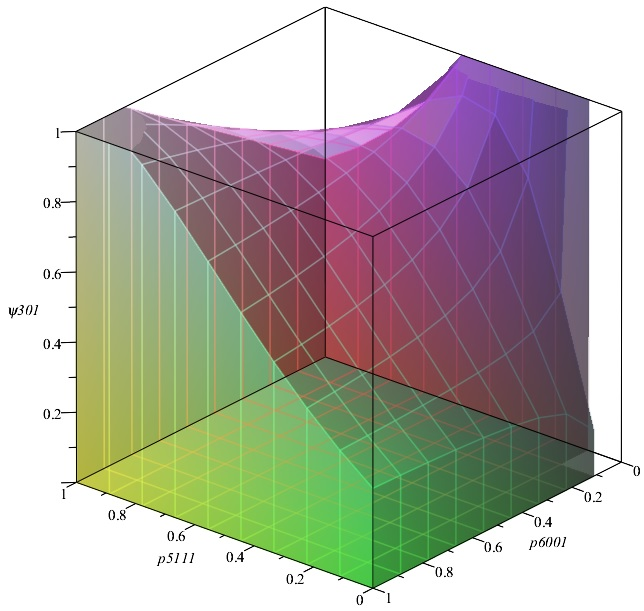
\includegraphics[scale=0.3]{ciaociao}}
\subcaptionbox{Optimal regions in the case $Y_3=0$.\label{fig:opt2}}
[.48\linewidth]{
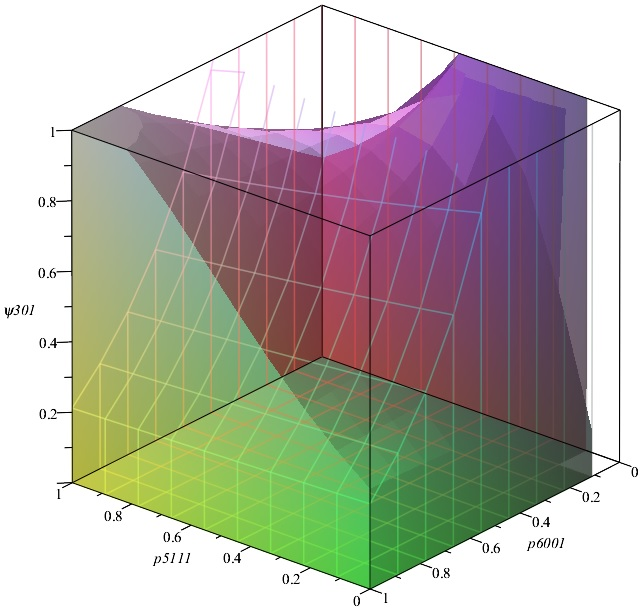
\includegraphics[scale=0.3]{ciaociao1}}
\end{center}
\caption{Regions determining the combinations of parameters leading to an optimal decision of evacuating (coloured regions) and not evacuating (white regions) for the evaluation of the diagram in Figure~\ref{fig-ex} given the partial numeric specification in Table~\ref{table:num}. \label{fig:opt}}
\end{figure}

Each of the above three operations changes the conditional expected utility vectors and their entries in a specific way we formalise below.

\begin{proposition}
\label{polyop}
For $i\in [n]$, let $\bar{\bm{u}}_{i+1}$ be a conditional expected utility vector whose entries have the polynomial structure of equation~(\ref{struct}) and let $u_j$ be the vertex preceding $Y_{i+1}$ in the DS. Then, in the notation of Theorem~\ref{polyexp},
\begin{itemize}
\item $\max^{\EU}_{\mathcal{Y}_i}\bar{\bm{u}}_{i+1}$ has dimension $c_{i+1}/r_i$ and its entries  do not change polynomial structure;
\item $\bar{\bm{u}}_{i+1} +^{\EU} \bm{\psi}_{j}$ has dimension $c_{i+1}s_{i}^\mathbb{U}$, where $s_i^\mathbb{U}=\prod_{k\in \{P_j\setminus B_{i+1}\}}r_k$, and each of its entries includes $r_{(i+1)ba}$ monomials of degree $d_{(i+1)ba}$, $r_{(i+1)ba}$ monomials of degree $d_{(i+1)ba}+3$ and one monomial of degree 2;
\item $\bar{\bm{u}}_{i+1}\Sigma^{\EU}\bm{p}_i$ has dimension $c_{i+1}s_i/r_i$, where $s_i=\prod_{k\in \{\Pi_i\setminus B_{i+1}\}}r_k$, and each of its entries includes $r_ir_{(i+1)ba}$ monomials of degree $d_{(i+1)ba}+1$.
\end{itemize} 
\end{proposition}
This result directly follows from the definition of the above three operations whose effect on the polynomials associated to the diagram in Figure~\ref{fig-ex} is illustrated below.

\subsubsection{A Fast Evaluation Algorithm.} \label{alg}
The algorithm for the evaluation of MIDs is given in Algorithm~\ref{algo}. This receives as input the DS of the MID, $S$ say, the sets $\mathbb{J}$, $\mathbb{V}$ and $\mathbb{D}$, and the vectors $\bm{p}=(\bm{p}_i)_{i\in[n]}^\T$, $\bm{\psi}=(\bm{\psi}_j)_{j\in[n]}^\T$ and $\bm{k}=(h,k_j)_{j\in[m]}^\T$. We implemented this algorithm in the \texttt{SymbolicExpectedUtility} function in Appendix \ref{appendixD}.\footnote{Note that the inputs of these functions in Maple are different. The ones chosen here are able to more concisely report their working.}.  This corresponds to a symbolic version of the backward induction procedure over the elements of the DS explicated in Proposition \ref{i-th}. At each  inductive step, a utility vertex is considered together with the variable that precedes it in the DS.

In line (1) the conditional expected utility $\bar{\bm{u}}_{n+1}$  is initialised to $(0)$.   
Lines (2) and (3) index a reverse loop over the indices of both the variables and the utility vertices respectively (starting from $n$ and $m$). If the current index corresponds to a variable preceding a utility vertex in the DS (line 4), then the algorithm jumps to lines (5)-(7). Otherwise it jumps to lines (8)-(10). In the former case, the algorithm computes, depending on whether or not the variable is controlled (line 5), either an \texttt{EUMaximisation} over $\mathcal{Y}_k$ (line 6) or an \texttt{EUMarginalisation} (line 7) with $\bm{p}_k$,  jointly to an \texttt{EUMultiSum} with $\bm{\psi}_l$. 
In the other case, \texttt{EUMaximisation} and \texttt{EUMarginalisation} operations are performed without \texttt{EUMultiSum}. 

\begin{figure*}
\begin{center}
\begin{spacing}{1.15}
\begin{pseudocode}[ruled]{SymbolicExpectedUtility}{\mathbb{J},S,\bm{p},\bm{\psi}, \bm{k},\mathbb{V},\mathbb{D}}
\label{algo}
\bar{\bm{u}}_{n+1}=(0)\hspace{10.79cm}(1)\\
\FOR k \GETS n \DOWNTO 1 \hspace{9.04cm}(2)\DO \BEGIN 
\FOR l \GETS m \DOWNTO 1 \hspace{7.74cm}(3)\DO \BEGIN
\IF k=j_l \hspace{8.67cm} (4)\THEN \BEGIN
\IF k\in \mathbb{D} \hspace{7.02cm}(5)\THEN\BEGIN
\bar{\bm{u}}_{k}=\max^{\EU}_{\mathcal{Y}_k}(\bar{\bm{u}}_{k+1}+^{\EU}\bm{\psi}_l)\hspace{2.22cm}(6)
\END
\ELSE \BEGIN
\bar{\bm{u}}_k=\bm{p}_k\;\Sigma^{\EU}\;(\bar{\bm{u}}_{k+1}+^{\EU}\bm{\psi}_{l}) \hspace{2.20cm}(7)
\END
\END
\ELSEIF k\in \mathbb{D} \hspace{7.56cm}(8)\THEN \BEGIN
\bar{\bm{u}}_k=\max^{\EU}_{\mathcal{Y}_k}\bar{\bm{u}}_{k+1}\hspace{5.46cm}(9)
\END
\ELSE \BEGIN
\bar{\bm{u}}_k=\bm{p}_k\;\Sigma^{\EU}_{\mathcal{Y}_k}\;\bar{\bm{u}}_{k+1}\hspace{5.31cm}(10)
\END
\END
\END\\
\RETURN{ \bar{\bm{U}}_{1}} \hspace{10.29cm} (11)
\label{algo1}
\end{pseudocode}
\end{spacing}
\end{center}
\vspace{-1.25cm}
\end{figure*}

\begin{example}
For the MID in Figure~\ref{fig-ex} the \texttt{SymbolicExpectedUtility} function first considers  the random vertex $Y_6$ which precedes the utility vertex $U_3$ and therefore first calls the \texttt{EUMultiSum} function. \texttt{EUDuplicationPsi} in this case entails that $\bar{u}_7$ is duplicated four times and 
\begin{equation}
\label{ms3}
\bar{\bm{U}}_7+^{\EU}\bm{\psi}_3=\left(
\begin{array}{cccc}
k_3\psi_{11}&
k_3\psi_{01}&
k_3\psi_{10}&
k_{3}\psi_{00}
\end{array}
\right)^\T.
\end{equation}
Then, the rhs of Equation~(\ref{ms3}) needs to be duplicated via \texttt{EUDuplicationP} and  
\begin{equation*}
\label{eq:ciao1}
\bar{\bm{u}}_6^\T=I'_6 \times \bar{\bm{u}}_6^t\circ \bm{p}_6= \left(k_3\psi_{31j}p_{61ij}+k_3\psi_{30j}p_{60ij}\right)_{i,j\in[1]^0}^\T,
\end{equation*}
where $\bar{\bm{u}}^t_6$ is equal to the duplicated version of the rhs of equation~(\ref{ms3}).
The vector $\bar{\bm{u}}_6$ has dimension four and its entries include two monomials of degree $3$. Since the random vertex $Y_5$ is the unique parent of $U_2$ the \texttt{SymbolicExpectedUtility} function follows the same steps as before. \texttt{EUMultiSum} is first called which gives as output
\begin{equation*}
\label{u6p}
\bar{\bm{u}}_6+^{\EU}\bm{\psi}_2= h\cdot k_2\cdot \bar{\bm{u}}_6\circ \left(
\begin{array}{cccc}
\psi_{21}&
\psi_{20}&
\psi_{21}&
\psi_{20}
\end{array}
\right)^\T+\bar{\bm{u}}_6+k_2\cdot\left(
\begin{array}{cccc}
\psi_{21}&
\psi_{20}&
\psi_{21}&
\psi_{20}
\end{array}
\right)^\T
\end{equation*}
The polynomial $\bar{\bm{u}}_6+^{\EU}\bm{\psi}_2$ is the sum of two monomials of degree $3$ inherited from $\bar{\bm{u}}_6$, of two monomials of degree $6$ (from the first term on the rhs of~\ref{u6p}) and one monomial of degree $2$ (from the last term on the rhs of~\ref{u6p}). Its dimension is equal to four (i.e. no \texttt{EUDuplicationPsi} is required). 
\texttt{EUMultiSum}  manipulates the conditional expected utility vector according to Proposition~\ref{polyop}. Then, the \texttt{EUMarginalisation} function computes
\[
\bar{\bm{u}}_5=
I_5'\times
\left(\left(\begin{array}{cc}
\bar{\bm{u}}_6+^{\EU}\bm{\psi}_2&
\bar{\bm{u}}_6+^{\EU}\bm{\psi}_2
\end{array}
\right)^\T\circ
\bm{p}_5\right).
\] 
Each entry of $\bar{\bm{u}}_5$ has twice the number of monomials of the entries of $\bar{\bm{u}}_6+^{\EU}\bm{\psi}_2$ and each  monomial of $\bar{\bm{u}}_5$ has degree $d+1$, where $d$ is the degree of each monomial of $\bar{\bm{u}}_6+^{\EU}\bm{\psi}_2$ (whose entries are homogeneous polynomials). These vectors also have the same dimension. Thus, this \texttt{EUMarginalisation} changes the conditional expected utility vector according to Proposition~\ref{polyop}. The polynomial in a generic entry of $\bar{\bm{u}}_5$ was shown in equations (\ref{u51})-(\ref{u52}).

The algorithm then considers the controlled variable $Y_4$. Since $4\not\in \mathbb{J}$, $Y_4$ is not the argument of a utility function with the highest index and therefore the algorithm calls the \texttt{EUMaximisation} function. Suppose the optimal decisions are identified to be $Y_4=1$ when $Y_3=1$ and $Y_4=0$ when $Y_3=0$. The evaluation would then suggest that the population is evacuated whenever a high level of deposition is observed and that people are not evacuated if the deposition is low. Then \texttt{EUMaximisation}  would  return $\bar{\bm{u}}_4=I^{*}_4\times \bar{\bm{u}}_5$, where $I^{*}_4$ is a $2\times 4$ matrix with ones in positions $(1,1)$ and $(2,4)$ and zeros otherwise.
Proposition~\ref{polyop} is respected since the entries of $\bar{\bm{u}}_4$ have the same polynomial structure of those of $\bar{\bm{u}}_5$ and $\bar{\bm{u}}_4$ has dimension $2$.

The \texttt{SymbolicExpectedUtility} function then applies in sequence the operations defined in  Section~\ref{op}. For the MID in Figure~\ref{fig-ex} it sequentially computes the following quantities:
\[
\begin{array}{ll}
\bar{\bm{u}}_3^t=h\cdot k_1\cdot \bar{\bm{u}}_4\circ\bm{\psi}_1
+\bar{\bm{u}}_4+ k_1\cdot 
\bm{\psi}_1,
& \bar{\bm{u}}_3 = I_3^{'}\times \left(\left(
\begin{array}{cccc}
\bar{\bm{u}}_3^t&
\bar{\bm{u}}_3^t&
\bar{\bm{u}}_3^t&
\bar{\bm{u}}_3^t
\end{array}
\right)^\T
\circ\bm{p}_3\right),\\
\bar{\bm{u}}_2=I_2^{'}\times
\left(\bar{\bm{u}}_3\circ
\bm{p}_2
\right),
&\bar{\bm{u}}_1=\left(
\begin{array}{cc}
1&0
\end{array}
\right)\times 
\bar{\bm{u}}_2,
\end{array}
\]
assuming the optimal initial decision is $Y_1=1$.

Interestingly, using the new algebra we introduced in Section~\ref{op}, the evaluation of an MID can be written as a simple algebraic expression. For example, the evaluation of the MID in Figure~\ref{fig-ex} can be written as
\begin{equation*}
\bar{\bm{U}}_1=\max\nolimits^{\EU}_{\mathcal{Y}_1}\Bigg(\bm{p}_2 \;\Sigma^{\EU}\;\bigg(\bm{p}_3\;\Sigma^{\EU}\;\Big(\bm{\psi}_1+^{\EU}\max\nolimits^{\EU}_{\mathcal{Y}_4}\big(\bm{p}_5\;\Sigma^{\EU}(\bm{\psi}_2+^{\EU}(\bm{p}_6\;\Sigma^{\EU}\bm{\psi}_3))\big)\Big)\bigg)\Bigg)
\end{equation*}
\end{example}
and this polynomial can be evaluated  with \texttt{SymbolicExpectedUtility}.

Although we have developed in this section a symbolic approach for the evaluation of extensive form MIDs, in \citet{Leonelli2015a} we formalise both the symbolic and the polynomial interpretation of the manipulations (edge reversal and barren node removal) of non extensive form diagrams. In that paper we further deduce the polynomial and symbolic interpretation of the sufficiency theorem of \citet{Smith1989}, that can be used to greatly simplify the evaluation of an MID by deleting some of its vertices.
 
\subsubsection{Asymmetric Decision Problems.}
\label{asymmetry}
In Section \ref{sec:asy} we claimed that most of the graphical representations of asymmetric decision problems lose the transparency associated to IDs. In this section we start to demonstrate one of the great advantages of symbolic approaches, namely that the complexity of both the polynomial structure and the symbolic definition of an asymmetric problem are simpler than the ones using a symmetric embedding of the problem. We discuss  this feature in greater length in Section \ref{sec:diff} below. 

Here we characterise an asymmetry between two chance nodes which, depending on the stage of the evaluation,  may  entail setting equal to zero monomials in either some or all rows of the conditional expected utility vector.  This therefore implies that the polynomial structure of the conditional expected utility vectors and at times also their dimension change. We present the result for elementary asymmetries of the following form: if $Y_i=y_i$ then $Y_j\neq y_j$, $i\neq j$ (see Section \ref{sec:asy} for an example of such asymmetries). Composite asymmetries are unions of simple asymmetries and the features of the conditional expected utility vectors in more general cases can be deduced through a sequential application of Theorem~\ref{polyasy}.

\begin{theorem}
\label{polyasy}
Let $\Gr$ be an MID, $Y_i$ and $Y_j$ be two random variables with $j>i$, $U_x$ be the first utility node that follows $Y_j$ in the DS. Assume the asymmetry $Y_i=y_i\Rightarrow Y_j\neq y_j$ holds and that $k$ and $z$ are the highest indices such that $j\in B_k$ and $i\in B_z$ and assume  $k>j$. Then 
\begin{itemize}
\item for $t\in[z]_j$, each row of $\bar{\bm{u}}_t$ has $\prod_{s\in B_t\setminus \{i\cup j\}} r_s$ rows with no monomials;
\item for $t\in[j]_i$, each row of $\bar{\bm{u}}_t$ has $\prod_{s\in B_t\setminus \{i\}} r_s$ rows with polynomials of a different structure. Specifically, these consists of, in the notation of Theorem~\ref{polyexp}, $r_{tba}'$ monomials of degree $d_{tba}$, where for $a\in[m]_{x-1}$ and $b\in[a]_{l-1}$ 
\[
r_{tba}'=\left(\binom{a-x}{b-l}-1\right)\prod_{s\in[j_a]_{t-1}}r_s/r_j;
\]  
\item for $t\in[i]$, each row of $\bar{\bm{u}}_t$ has in the notation of Theorem~\ref{polyexp} $r_{tba}''$ monomials of degree $d_{tba}$, where for $a\in[m]_{x-1}$ and $b\in[a]_{l-1}$ 
\[
r_{tba}''=\left(\binom{a-x}{b-l}-1\right)\prod_{s\in[j_a]_{t-1}}r_s/(r_j\cdot r_i).
\]  
\end{itemize}

\end{theorem}
The proof of this theorem is provided in Appendix \ref{cippu}.
{Corollary~\ref{corro} gives a  characterisation of simple asymmetries between any two variables, whether they are controlled or non-controlled. This follows  from Theorem~\ref{polyasy} since controlled variables can be thought of as a special case of random ones.

\begin{corollary}\label{corro}
In the notation of Theorem~\ref{polyexp} and under the assumptions of Theorem~\ref{polyasy}, with the difference that $Y_i$ and $Y_j$ are two variables, controlled or non-controlled, we have that
\begin{itemize}
\item for $t\in[z]_j$, each row of $\bar{\bm{u}}_t$ has $\prod_{s\in B_t\setminus \{i\cup j\}} r_s$ rows with no monomials;
\item for $t\in[j]_i$, $\bar{\bm{u}}_t$ has at most $\prod_{s\in B_t\setminus \{i\}} r_s$ rows with polynomials of a different structure. Specifically, these consists of between $r_{tba}'$ and $r_{tba}$ monomials of degree $d_{tba}$, for $a\in[m]_{x-1}$ and $b\in[a]_{l-1}$;
\item  for $t\in[i]$, some rows of $\bar{\bm{u}}_t$ have a number of monomials of degree $d_{tba}$ between $r_{tba}''$ and $r_{tba}$, for $a\in[m]_{x-1}$ and $b\in[a]_{l-1}$.
\end{itemize} 
\label{corasy}
\end{corollary}


\begin{example}[Example~\ref{eee} continued]
 Consider the asymmetric problem described in Figure \ref{sid}. The symbolic imposition of the asymmetric constraints reduces from ten to three the number of monomials in $\bar{u}_5$ which becomes 
\[
k_3\psi_{311}p_{6111}p_{511i}+k_2\psi_{21}p_{511i}+hk_2k_3\psi_{311}\psi_{21}p_{6111}p_{511i}, \;\;\;\;\; i\in[1]^0.
\]
Suppose the \texttt{EUMaximisation} suggested that $Y_4=0$ is optimal if $Y_3=1$ and that $Y_4=1$ is preferred if $Y_3=0$. The entry of $\bar{u}_3$ for which $Y_2=1$ and $Y_1=1$ can be written as
\begin{multline*}
\sum_{i,\in[1]^0}((k_2\psi_{21}+k_3\psi_{311}p_{6111}(1+hk_2\psi_{21}))p_{5110}p_{3011}+k_1\psi_{1i}p_{3i11}\\
+hk_1k_3\psi_{11}p_{5101}p_{3111}((1+k_2\psi_{21})\psi_{3j0}p_{6j10})).
\end{multline*}
This polynomial consists of only nine monomials. This, compared with the number of monomials in the symmetric case, 42,  means that even in this small problem we obtain a reduction  of the number of monomials by over three quarters.
\end{example}

So the example above illustrates that under asymmetries the polynomial representation is simpler than standard methods but still able to inform decision centres about the necessary parameters to elicit.  Finally, it is possible to develop a variant of Algorithm~\ref{algo1} which explicitly takes into account the asymmetries of the problem \textit{during} its evaluation.  Note that this approach  would  be  computationally even more efficient, since it would require the computation of a smaller number of monomials/polynomials.
 
\subsection{A Differential Approach to Inference in Staged Trees}
\label{sec:diff}

\subsubsection{Symbolic Definition of Staged Trees.}
As discussed in Section \ref{sec:history}, symbolic methods have proved useful in the study of BNs, despite coming with a considerable computational cost. In this section we develop a symbolic approach for \textit{staged trees} \citep[see e.g.][and Section \ref{sec:tree}]{Smith2008} and we demonstrate that such difficulties are eased, because of the more intuitive parametrisation associated to these models. In addition, because of the wide variety of possible hypotheses they embody, staged trees are necessarily models over much smaller state spaces than BNs. Since the size of the model space is the main computational issue for symbolic approaches associated with BNs, it follows that trees can be very practical contexts to investigate symbolic inferential queries.

Borrowing ideas from  \citet{Pistone2001}, we define the \textit{interpolating polynomial} of a staged tree.

\begin{definition}\label{def:interpol}
Let $\mathcal{T}=(V,E)$ be a staged tree with primitive probabilities $\theta_e$, $e\in E$, and set of root-to-leaf paths $\Lambda(s_0,\mathcal{T})$. We call $\Lambda(e)=\{r\in\Lambda(s_0,\mathcal{T})\;|\; e\in E(r)\}$ an \emph{edge centred} event, and set 
$\lambda_e(r)$, for $e\in E$, to be an indicator of $r\in\Lambda(e)$. We call
\begin{equation*}\label{eq:interpol}
c_{\mathcal{T}}(\theta,\lambda)=\sum_{\mathclap{r\in R_\mathcal{T}~}}~\prod_{\mathclap{\quad e\in E(r)}}\lambda_e(r)\theta_e
\end{equation*}
the \textbf{interpolating polynomial} of $\mathcal{T}$.
\end{definition}

The interpolating polynomial is a sum of probabilities of atomic events with indicators for certain conditional events happening or not happening. Even though all these unknowns sum to one, in our symbolic approach we treat them just like indeterminates. Note that the indicators $\lambda_e(r)$ on the edges $e\in E(r)$ are associated to the (conditional) event represented by $e$, having probability $\theta_e$. This notation is apparently redundant, but turns out to be useful below. We observe that this redundancy is one of the great advantages of a staged tree: whilst \cite{Darwiche2003} needs to compute conditional probabilities of all \emph{compatible parent structures} of an event, which is a rather obscure concept in a symbolic framework, and \cite{Castillo1996a} computes the product space of any indeterminates' combination regardless of their meaning, a tree visualisation of our model gives us the necessary structure immediately: events can be simply read from the paths in the graph. 

\begin{example}
The interpolating polynomial of the tree in Figure \ref{fig:ET} (on page \pageref{riporto}), not considering the underlying stage structure, is equal to (for ease of notation we omit the indicator functions) 
\begin{equation}\label{eq:interpolstaged}
c_\mathcal{T}'(\theta)=\theta_{01}\theta_{11}\theta_{31}
+\theta_{01}\theta_{11}\theta_{30}
+\theta_{01}\theta_{10}\theta_{41}
+\theta_{01}\theta_{10}\theta_{40}
+\theta_{00}\theta_{21}
+\theta_{00}\theta_{20}.
\end{equation}
When plugging in the conditional independence constraints, we obtain the interpolating polynomial of the staged tree as
\begin{align}\label{eq:interpolceg}
c_\mathcal{T}(\theta)&=\theta_{01}\theta_{11}\theta_{31}
+\theta_{01}\theta_{11}\theta_{30}
+\theta_{01}\theta_{10}\theta_{31}
+\theta_{01}\theta_{10}\theta_{30}
+\theta_{00}\theta_{11}
+\theta_{00}\theta_{10},\\
&~=~\theta_{01}(\theta_{11}(\theta_{31}+\theta_{30})+\theta_{10}(\theta_{31}+\theta_{30}))+\theta_{00}(\theta_{11}+\theta_{10}).\label{eq:factored}
\end{align}
Conversely, the interpolating polynomial of the BN representation of the problem described by this staged tree, ignoring the conditional independence structure, equals 
\begin{equation}\label{eq:interpolBN}
\begin{split}
c_{\text{BN}}(\theta)=&
\theta_{01}\theta_{11}\theta_{31}
+\theta_{01}\theta_{11}\theta_{30}
+\theta_{01}\theta_{10}\theta_{41}
+\theta_{01}\theta_{10}\theta_{40}\\
&+\theta_{00}\theta_{21}\theta_{51}
+\theta_{00}\theta_{21}\theta_{50}
+\theta_{00}\theta_{20}\theta_{61}
+\theta_{00}\theta_{20}\theta_{60},
\end{split}
\end{equation}
\end{example}

We now look at interpolating polynomials from an algebraic viewpoint. Because of the product space structure of the sample space of a BN, the interpolating polynomial of a BN with $n$ vertices equals the sum of  monomials each of which is of degree $2n$ and so \emph{homogeneous}. Moreover, the stage structure of a tree associated to a BN model as in Figure \ref{fig:ETBN} is such that no two vertices along the same directed path are in the same stage, in fact stages exist only along \emph{orthogonal cuts} \citep{Thwaites2015}. Thus, the interpolating polynomial of a BN is also square-free. This is shown for instance by the interpolating polynomial $c_{\text{BN}}$ in equation (\ref{eq:interpolBN}),  an homogeneous polynomial of degree $3$ whose number of terms equals the number of paths in its tree representation.  Importantly this polynomial has been simply read from the event tree by first multiplying over all primitive probabilities along one root-to-leaf path, and then summing over all of these paths. This is a lot easier done using Figure \ref{fig:ETBN} (on page \pageref{fig:ETBN}) than in the associate BN representation, where we would have had to sum over compatible parent configurations.

Conversely, interpolating polynomials of staged trees are not necessarily homogeneous and  square-free. For instance, the interpolating polynomial in equation (\ref{eq:interpolceg}) is now inhomogeneous with total degree $3$ and monomial terms having degree $2$ and $3$. Although our staged tree examples have a square-free structure, non multilinear interpolating polynomials arise from a tree where two vertices  in the same root-to-leaf path are in the same stage \citep[as shown in][]{Gorgen2015}. For the purpose of this section we focus only on staged trees whose interpolating polynomial is square-free.

 Notice that $c_\mathcal{T}$ can be easily factorised in equation (\ref{eq:factored}) by simply following the structure of the underlying graph. In \cite{Brandherm2004} polynomials of this type are called \textit{factored}. This representation entails great computational advantages since the compilation into an AC is almost instantaneous. Whilst for BNs the factored representation might be difficult to obtain, it comes almost for free in tree models. 

We observe that the graphical simplicity of  staged tree models in comparison to an uncoloured tree or trees associated to BNs is also reflected algebraically: the polynomial in (\ref{eq:interpolceg}) has fewer indeterminates than the one in (\ref{eq:interpolstaged}) and a lot fewer than the polynomial associated to a tree which is derived from a BN in (\ref{eq:interpolBN}). This is because in the BN the redundancy of atoms gives rise to redundant terms. 

The definition of interpolating polynomials enables us to compute the probability of any event associated to a tree. 
\begin{lemma}\label{lem:darwiche}
For any event $A$ represented by a set of root-to-leaf paths $R_A$ in a staged tree $\mathcal{T}$,
\begin{equation*}\label{eq:lem1}
\mathbb{P}(A)=\sum_{\mathclap{r\in R_A~}}~\prod_{\mathclap{\quad e\in E(r)}}\lambda_e(r)\theta_e=c_\mathcal{T}(\theta,\lambda|_{R_A}),
\end{equation*}
where $\lambda|_{R_A}$ indicates that $\lambda_e(r)=1$ for all $e\in E(r)$ with $r\in R_A$, and else zero.
\end{lemma} 
This result holds since the probability of an event is equal to the sum of the probabilities of the associated root-to-leaf paths.

\begin{example}\label{bsp:lem1}
Suppose we are interested in calculating the probability of  political disruption. This is captured by the set $R_A=\Lambda(e_{31})\cup\Lambda(e_{41})$ corresponding to all root-to-leaf paths going through an edge labelled \lq{y}es', which translates in  summing all terms in (\ref{eq:interpolceg}) including $\theta_{31}$. Therefore $\mathbb{P}(A)=\theta_{01}\theta_{11}\theta_{31}+\theta_{01}\theta_{12}\theta_{31}$, again omitting the $\lambda$ indicators.
\end{example}

\subsubsection{The Differential Approach.}\label{sect:diff}
We are now able to provide a probabilistic semantic, just as \cite{Darwiche2003} for BNs, to the derivatives of  polynomials associated to staged trees. For ease of notation we let in this section $\lambda_e=\lambda_e(r)$.

\begin{proposition}\label{prop:darwiche}
For equally coloured edges $e\in E$ and an event $A$ represented by the root-to-leaf paths $R_A$, it holds that
\begin{equation}
\label{eq:der1}
\mathbb{P}(\Lambda(e)\;|\;A)=\frac{1}{c_\mathcal{T}(\theta,\lambda|_{R_A})}\frac{\dr c_\mathcal{T}(\theta,\lambda|_{R_A})}{\dr \lambda_e},~\;\;\;
\mathbb{P}(\Lambda(e),A)=\theta_e\frac{\dr c_\mathcal{T}(\theta,\lambda|_{R_A})}{\dr \theta_e}.
\end{equation}
\end{proposition}
\begin{proof}
First consider the equation on the left. Recall that $\mathbb{P}(\Lambda(e)\;|\;A)=\frac{\mathbb{P}(\Lambda(e),A)}{\mathbb{P}(A)}$. From Lemma \ref{lem:darwiche} it follows that the denominator is as in (\ref{eq:der1}). For the numerator note that 
\[
\frac{\dr c_\mathcal{T}(\theta,\lambda|_{R_A})}{\dr \lambda_e}=\frac{\dr \sum_{r\in R_A}\prod_{ e\in E(r)}\lambda_e(r)\theta_e}{\dr \lambda_e}=\sum_{r\in\Lambda(e)\cap R_A}\prod_{a\in E(r)}\lambda_a\theta_a=\mathbb{P}(\Lambda(e),A),
\]
from which the equation on the left follows. Finally note that 
\[
\theta_e\frac{\dr c_\mathcal{T}(\theta,\lambda|_{R_A})}{\dr \theta_e}=\frac{\dr c_\mathcal{T}(\theta,\lambda|_{R_A})}{\dr \lambda_e},
\]
since $\lambda_e$ is equal to either one or zero, depending on whether a root-to-leaf path in $R_A$ goes through $e$ or not.  
\end{proof}

 Notice that the derivatives of tree polynomials have the exact same interpretation of the ones of BNs as in \cite{Darwiche2003}. Here we restricted our attention to square free staged trees but analogous results hold in the generic case: each monomial with indeterminates $\lambda_e$ and $\theta_e$ of degree higher than one would need to be differentiated a number of times equal to the degree of that indeterminate.

\begin{proposition} \label{prop:darwiche2}
In the notation of Proposition \ref{prop:darwiche}, the following holds for $e,e_1, e_2\in E$:
\begin{align}
\mathbb{P}(\Lambda(e_1),\Lambda(e_2)\;|\; A)&~=~ \frac{1}{c_\mathcal{T}(\theta,\lambda|_{R_A})}\frac{\partial^2 c_\mathcal{T}(\theta,\lambda|_{R_A})}{\partial \lambda_{e_1}\partial\lambda_{e_2}}, \label{eq:diff1}\\
\mathbb{P}(\Lambda(e_1),\Lambda(e_2),A)&~=~\theta_{e_1}\theta_{e_2}\frac{\partial c_\mathcal{T}(\theta,\lambda|_{R_A})}{\partial \theta_{e_1}\partial \theta_{e_2}},\label{eq:diff2}\\
\mathbb{P}(A\;|\; \Lambda(e))&~=~\frac{\partial^2 c_\mathcal{T}(\theta,\lambda|_{R_A})}{\partial \theta_e \partial \lambda_e}.\label{eq:diff3} 
\end{align}
\end{proposition}
\begin{proof}
Equations (\ref{eq:diff1}) and (\ref{eq:diff2}) follow applying twice equation (\ref{eq:der1}). To prove (\ref{eq:diff3}), note that
\[
\mathbb{P}(A\;|\;\Lambda(e))=\frac{\mathbb{P}(A,\Lambda(e))}{\mathbb{P}(\Lambda(e))}=\frac{\dr c_\mathcal{T}(\theta,\lambda|_{R_A})}{\dr \lambda_e}\frac{1}{\theta_e}=\theta_e\frac{\dr c_\mathcal{T}(\theta,\lambda|_{R_A})}{\dr \theta_e}\frac{1}{\theta_e}=\frac{\dr^2c_\mathcal{T}(\theta,\lambda|_{R_A})}{\dr \theta_e \dr \lambda_e}.
\]
\end{proof}
It is easy to then deduce from Proposition \ref{prop:darwiche2} the probabilistic meaning of higher order derivatives.

Importantly, in the staged tree model class derivatives can be associated to causal propositions. Note that such a result does not hold in general for the polynomials describing BN probabilities. 

\begin{proposition}
Suppose the staged tree is believed to be causal as in \citet{Thwaites2010}. Then in the notation of Proposition \ref{prop:darwiche2},
\begin{equation}
\label{eq:causal}
\mathbb{P}(A\;||\; \Lambda(e))=\frac{\partial^2 c_\mathcal{T}(\theta,\lambda|_{R_A})}{\partial \theta_e \partial \lambda_e},
\end{equation}
where $\mathbb{P}(A\;||\; \Lambda(e))$ is the probability of the event $A$ when the system is forced to go through the edge $e$.
\end{proposition}
\begin{proof}
This follows noting that in a causal framework $\mathbb{P}(A\;||\; \Lambda(e))=\mathbb{P}(A\;|\; \Lambda(e))$.
\end{proof}
Note that all the quantities in (\ref{eq:der1})-(\ref{eq:causal}) can be used in sensitivity analysis. For instance we could investigate the changes in probability estimates when the system is set to be in a certain scenario of interest.

\begin{example}\label{bsp:derivatives}
We now compute a set of derivatives of the interpolating polynomial $c_\mathcal{T}$ in (\ref{eq:interpolceg}) with respect to $\lambda_{31}$ and $\theta_{31}$ to perform probabilistic inference over the event $A$ of political disruption. Thus, we consider the edge $e=(v_3,v_7)$ and
\begin{align}
\frac{1}{c_\mathcal{T}(\theta,\lambda|_{R_A})}\frac{\dr c_\mathcal{T}(\theta,\lambda|_{R_A})}{\dr \lambda_e}&~=~\frac{\theta_{01}\theta_{11}\theta_{31}+\theta_{01}\theta_{12}\theta_{31}}{\theta_{01}\theta_{11}\theta_{31}+\theta_{01}\theta_{12}\theta_{31}}=1,\label{eq:1deriv_lambda}\\
\theta_e\frac{\dr c_\mathcal{T}(\theta,\lambda|_{R_A})}{\dr \theta_e}&~=~\theta_{13}(\theta_{01}\theta_{11}+\theta_{01}\theta_{12})=\mathbb{P}(A)\label{eq:1deriv_theta},\\
\frac{\dr^2 c_\mathcal{T}(\theta,\lambda|_{R_A})}{\dr \theta_e \dr \lambda_e}&~=~\theta_{01}\theta_{11}+\theta_{01}\theta_{12}.\label{eq:2deriv_lambdatheta}
\end{align}
Observe that equation (\ref{eq:1deriv_lambda}) is equal to one since every path associated to the event $A$ must go through $e$. From the same argument it follows that equation  (\ref{eq:1deriv_theta}) is equal to $\mathbb{P}(A)$. Equation (\ref{eq:2deriv_lambdatheta}) is a simple consequence of Bayes theorem, which can be checked algebraically. 
\end{example}

\subsubsection{Trees as Circuits.}\label{sect:circuit}
The previous sections have introduced a comprehensive symbolic inferential toolbox for trees, based on the computation of the interpolating polynomial and its derivatives. In \cite{Darwiche2003} it is shown that an efficient method to compute such polynomials is by representing them as an \textbf{AC}. This is a DAG whose leaves are the indeterminates and the inner nodes are labelled by multiplication and summation operations. The \emph{size} of  the circuit is measured by its number of edges.

ACs of staged tree polynomials are smaller in size than the ones associated to BNs for two reasons: first, a tree might have fewer root-to-leaf paths (as in our example); second, there can be less indeterminates because unfoldings with probability zero are not included in the model and coloured labels further decrease the number of indeterminates. Therefore, in asymmetric settings we can expect computations to be much faster for trees than BNs.

A major problem in the compilation of BNs polynomials consists of the identification of the AC of smallest size. This usually entails the computation of the BN's jointree and the application of rather complicated algorithms \citep{Darwiche2003}. We note here that in tree models this is straightforward since the interpolating polynomial is naturally factored.

\begin{example}
Notice that equation (\ref{eq:factored}) can be rewritten as
$
c_\mathcal{T}(\theta)=\theta_{01}(\theta_{11}+\theta_{12})(\theta_{31}+\theta_{31})+\theta_{02}(\theta_{11}+\theta_{12}).
$ This gives us the AC in Figure \ref{fig:arthcirc} where leaves with the same parent are labelled by primitive probabilities from the same floret, and labels belonging to leaves in the tree are first summed in the AC. It is easy to deduce that the AC associated to the BN's polynomial in equation (\ref{eq:interpolBN}) would be much larger than the one in Figure \ref{fig:arthcirc}. We note also that, whilst all the ACs deriving from BNs in \cite{Darwiche2003} are trees, ours are more generally DAGs. This is a consequence of the more flexible stage structure associated to generic staged trees than the one of trees depicting BNs. 

\begin{figure}[tb]
\[\xymatrixcolsep{0.7pc}\xymatrixrowsep{0.2pc}{\xymatrix{
&&&& +\ar[ld]\ar[rrd]\\
&&& \star\ar[llld]\ar[ld] \ar[drr]&&& \star\ar[ld]\ar[rd] \\
\theta_{01}&& +\ar[ld]\ar[rd] &&& +\ar[ld]\ar[rd] &&\theta_{02}\\
&\theta_{31}&&\theta_{32}&\theta_{11}&&\theta_{12}
}}\]\vspace*{-10pt}%reducing extra space caused by \[...\]
\caption[]{The arithmetic circuit of the polynomial in equation (\ref{eq:interpolceg}).}\label{fig:arthcirc}
\end{figure}
\end{example}

\section{Conclusions}
In this chapter, after discussing the links between algebraic and symbolic inferential methods, we have developed formal algebraic methods to investigate adequacy in IDSSs. We have defined new separation conditions consisting of certain polynomial relations and demonstrated that these can guarantee adequacy and distributivity in general and in a variety of examples. In particular, the application of such methods to the class of BN models defined as DAG linear regressions lead us to deduce new formulae for the computation of moments of not only additive, but also multilinear, functions of random vectors over an agreed DAG. We have then extended current symbolic inferential methods to IDs and staged trees. For IDs we have defined a new symbolic representation of utilities, introduced a new symbolic evaluation algorithm and discussed asymmetric constraints in symbolic frameworks. Concerning staged trees, we have developed an inferential approach based on the computation of the derivatives of probability polynomials. 
